% Activate the following line by filling in the right side. If for example the name of the root file is Main.tex, write
% "...root = Main.tex" if the chapter file is in the same directory, and "...root = ../Main.tex" if the chapter is in a subdirectory.
 
% !TEX root = ../thesis.tex 

\chapter{Cortical surface projection of volumetric data}
\label{projection_chapter}

\section{Introduction}

Surface-based methods can offer advantages for the analysis of physiological imaging data from particular anatomical structures. As applied to the cortex, previous work has shown that they can facilitate improved localisation of functional areas within subjects and better registration between subjects compared to conventional volumetric methods \cite{Glasser2016, Coalson2017}. Whilst some modalities lend themselves naturally to surface-based analysis (notably EEG), those that acquire volumetric data require an extra processing step to transform the data into the surface space. This is true of all MRI based methods, including BOLD fMRI (for which a number of projection methods exist), and ASL (for which little prior work exists that is specific to the modality). 

The projection framework that is developed in this chapter (incorporated into the Toblerone package and hereafter referred to by that name) is intimately tied to the combined surface and volumetric inference framework that will be introduced in chapter \ref{svb_chapter}. Whilst it can be used as a standalone tool in a manner comparable to existing methods, the principles on which it is built (in particular, hybrid space) are best understood in the context of the analysis framework that will follow. 


\subsection{Objectives}

Three existing projection methods for BOLD fMRI were introduced in section \ref{lit_projection_methods}. Whilst any of these could in principle be made to operate with other modalities, such as ASL, they all share the common property of encoding assumptions about the BOLD signal within their formulations. This is of vital importance as the assumptions cannot necessarily be carried across to other modalities. Considering ASL, for example, the point of divergence is signal from WM. In BOLD, it is assumed that little signal originates in WM, and that which does is often treated as noise. For a modality such as ASL, WM does generate a signal of interest (albeit weaker and therefore more difficult to analyse than GM), and it should therefore not be neglected or discarded. Furthermore, the space in which analysis is performed is of vital importance: though it  makes sense to analyse cortical signal in a surface-based manner, this is not true of WM signal, and so what is ultimately required is projection framework that both acknowledges the existence of signals arising from multiple tissues, \textit{and} allows for the analysis of these signals in the space that is best suited for them (cortical on the surface, subcortical in the volume).  

Whilst the core of this framework shares many features in common with the HCP's ribbon-constrained (RC) method, a number of important changes have been made. The end result can be used in two different ways. Firstly, it can be used in a narrow sense to perform volume-surface projection in a manner comparable to RC (and offering small improvements in performance). Secondly, it can be used in its novel form to project data to and from a hybrid space as part of a process of parameter estimation. Used in this manner, significant improvements in performance compared to the RC method are observed, though it is acknowledged that the comparison is imperfect as the RC method is not designed for this purpose. 

\subsection{Hybrid space}

The terms \textit{volume}, \textit{surface} and \textit{hybrid} space will be used throughout this chapter. These are used to refer to the space of representation of data. For example, voxel-wise data is in volume space; vertex-wise data on the cortical surface is in surface space; and data that has both a voxel- and vertex-wise representation is in hybrid space. 

The concept of hybrid space is of fundamental importance to this projection framework. It follows directly from the aforementioned use case for this method, which is to perform physiological parameter estimation for both the cortex and subcortex simultaneously, hereafter referred to as \textit{hybrid inference}. The spatial locations within the brain at which estimation is to be performed are termed \textit{nodes}, hence, within hybrid space the set of all nodes is defined as all surface vertices ($\vec{p}_L$ and $\vec{p}_R$ for the left/right hemispheres of the cortex) and all voxels ($\vec{v}$) of interest. 

\begin{equation}
\vec{n} = [\ \vec{p}_L \ | \ \vec{p}_R \ | \ \vec{v} \ ] 
\end{equation} 

Hybrid space permits parameter estimation in the space most suited to the structure in question: cortical parameters are estimated on the surface and subcortical parameters are estimated within voxel space. As far as is permitted by the available anatomical information (surface segmentations and volumetric masks), the defining principle of hybrid space is that each node should only correspond to one tissue. Voxels that contain both cortical and subcortical partial volumes will therefore contain \textit{multiple} nodes: one for each surface vertex and one for the voxel centre itself. This is an embodiment of the partial volume effect (the presence of multiple sources in a single voxel) and is illustrated in figure \ref{voxel_node}. The CIFTI file format \cite{cifti} embodies a similar principle to this definition of hybrid space, whereby cortical data is stored in a vertex-wise manner on the surface and subcortical data is stored in a voxel-wise manner, all within the same structure.

\begin{figure}
\centering
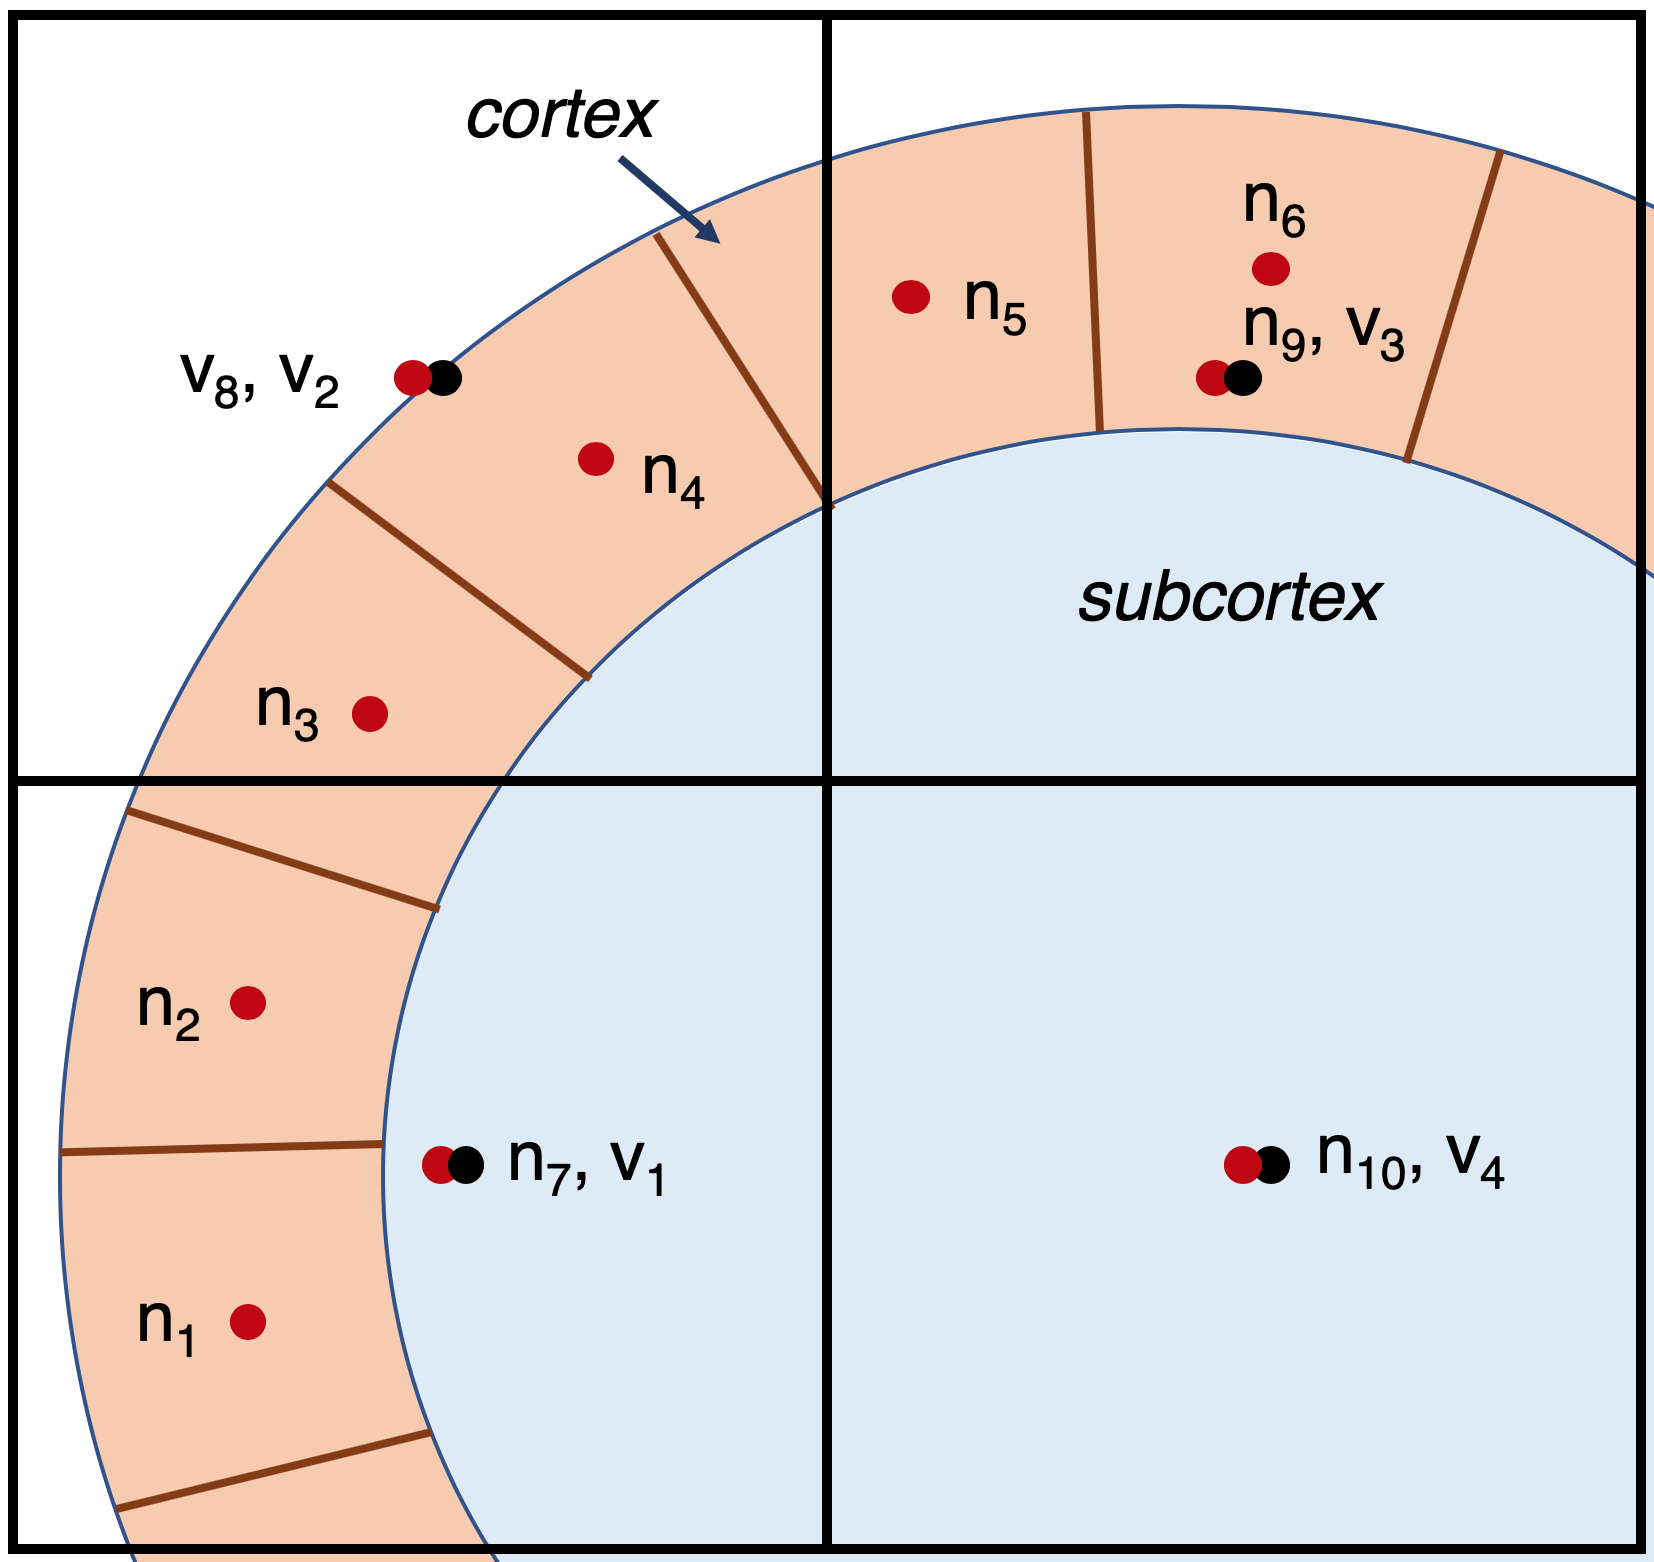
\includegraphics[width=0.5\textwidth]{voxel_node.png}
\caption{Schematic representation of voxels and nodes. The primitives comprising the cortical ribbon are denoted with brown boundaries. Voxel boundaries and centres are in black, labelled $v_1$ to $v_4$. Nodes are in red; $n_1$ to $n_6$ are cortical (corresponding to surface vertices), $n_7$ to $n_{10}$ are subcortical (corresponding to voxels). Individual voxels may contain multiple nodes, which is an explicit representation of PVE.}
\label{voxel_node} 
\end{figure}

As nodes in hybrid space correspond to only one tissue, the signals associated with them must also respect this distinction. Signal on cortical nodes is considered as being purely cortical (i.e., GM) in origin, and signal on subcortical nodes is considered as purely subcortical in origin (i.e., WM or a subcortical GM structure). \textit{How} these separate signals are derived from data that contains PVE is beyond the scope of this chapter (and is in fact the objective of PVEc)\footnote{Though many projection methods acknowledge the existence of PVE within data, there is little that can be done to rectify this during the narrow operation of projection. To do so would require a basis on which to separate cortical and subcortical contributions, which is the purpose of PVEc itself and therefore a non-trivial operation.}. For the purposes of this work, it is only necessary to posit that the separate signals exist and that their representation respects their separation. When projecting from hybrid to volume space, the process of PVE must therefore be recreated to mix the separate signals within each voxel. It is this specific projection, incorporating PVE, which facilitates the performance of surface-aware parameter estimation as it allows for the reconstruction of volumetric data from a set of cortical and subcortical parameter estimates. This will be addressed in chapter \ref{svb_chapter}. 

Whilst projection to and from hybrid space, for the purpose of performing hybrid inference, is the intended use case of the work presented in this chapter, Toblerone's projection can be made to operate in a conventional surface-volume sense. In this form, a projection that is directly comparable to existing surface-volume methods is recovered. 

\section{Construction of the projection}

The projections described herein can be performed with either one or both cortical hemispheres at a time. The forward and reverse projections are constructed from the same two matrices. Conceptually, these perform a transformation between voxels and surface triangles, and then between surface triangles and surface vertices. The cortical midsurface (exactly halfway in between the white and pial surfaces) is used by default, though this could be modified for other use cases (such as laminar fMRI). A set of PV estimates for the cortex is also used; these are produced using Toblerone's PV estimation function operating on the cortical surfaces, as detailed in chapter \ref{tob_pv_chapter}.

\subsection{Voxel-triangle matrix}
The voxel-triangle matrix records the intersection between individual voxels and the volume primitives that comprise the cortex. The problem is approached in a triangle-wise manner, as opposed to vertex-wise, as this allows for the construction of extremely simple primitives. Triangle correspondence between the inner (white) and outer (pial) surfaces of the cortex is assumed. For each pair of triangles, their corresponding vertices are connected to form a triangular prism\footnote{Or, even better, a Toblerone bar, hence the name.} which is then subdivided into three non-overlapping tetrahedra \cite{Dompierre1999}. For example, for triangles with vertices $\triangle ABC$ and $\triangle abc$ on the pial and white surfaces respectively, the prism may be split as $ABCa$, $Cabc$ and $BCab$. As a consequence of this subdivision, each rectangular face of the prism will be split along the diagonal into two triangles. It is important to ensure that the orientation of this face diagonal is consistent between neighbouring prisms so as to avoid producing overlapping tetrahedra. This is achieved by fixing the direction of subdivision according to the ordering of vertex numbers: `positive' if $A < B$, $B < C$ or $C < A$, and `negative' otherwise. 

Subsequently, for each voxel in the neighbourhood of the prism, an isotropic grid of sample points is initialised. Figure \ref{prism} shows one such prism and the sample points from one neighbourhood voxel. These points are tested to determine if they lie within each tetrahedra (via the Delaunay triangulation \cite{Barber:1996:QAC:235815.235821}) and the fraction that do are recorded in $\mat{VT}$, a matrix sized (voxels x triangles). 

\begin{equation}
\mat{VT} = 
\begin{bmatrix}
vt_{11} & \ldots & vt_{1t} \\
\vdots & \ddots & \vdots \\
vt_{v1} & \ldots & vt_{vt}
\end{bmatrix}
\end{equation}

The elements $vt_{vt}$ are continuous values in the range [0,1] recording the fraction of sample points from voxel $v$ that lie inside triangular prism $t$. This matrix is highly sparse: for a voxel size of 2.2mm isotropic and a surface resolution of 32k vertices, each triangular prism intersects around 10 voxels on average.

\begin{figure}[H]
\centering
\subcaptionbox{\label{prism1}}[0.45\textwidth]
{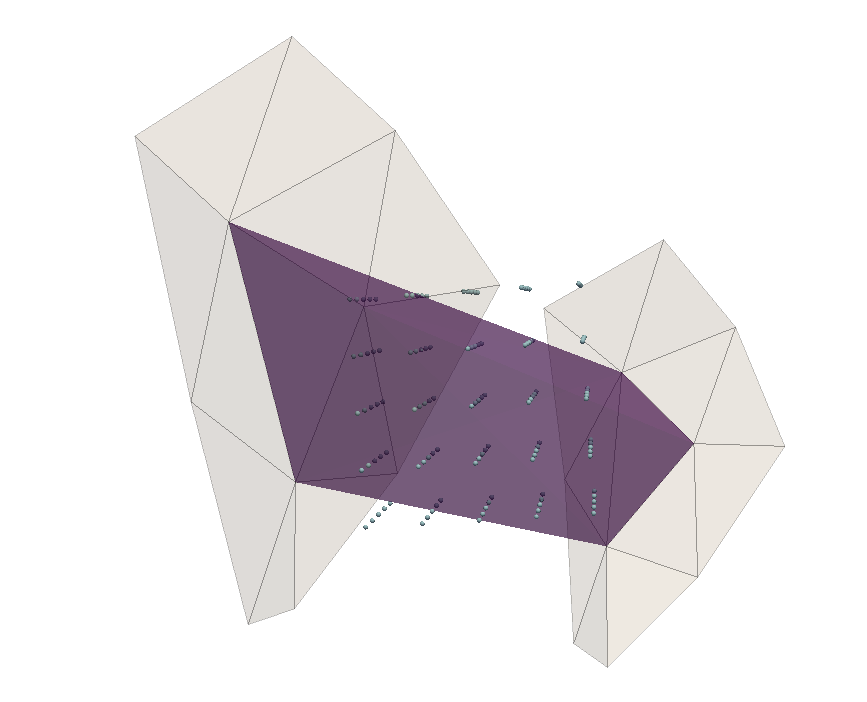
\includegraphics[width=0.45\textwidth]{prism4}}
\subcaptionbox{\label{prism2}}[0.45\textwidth]
{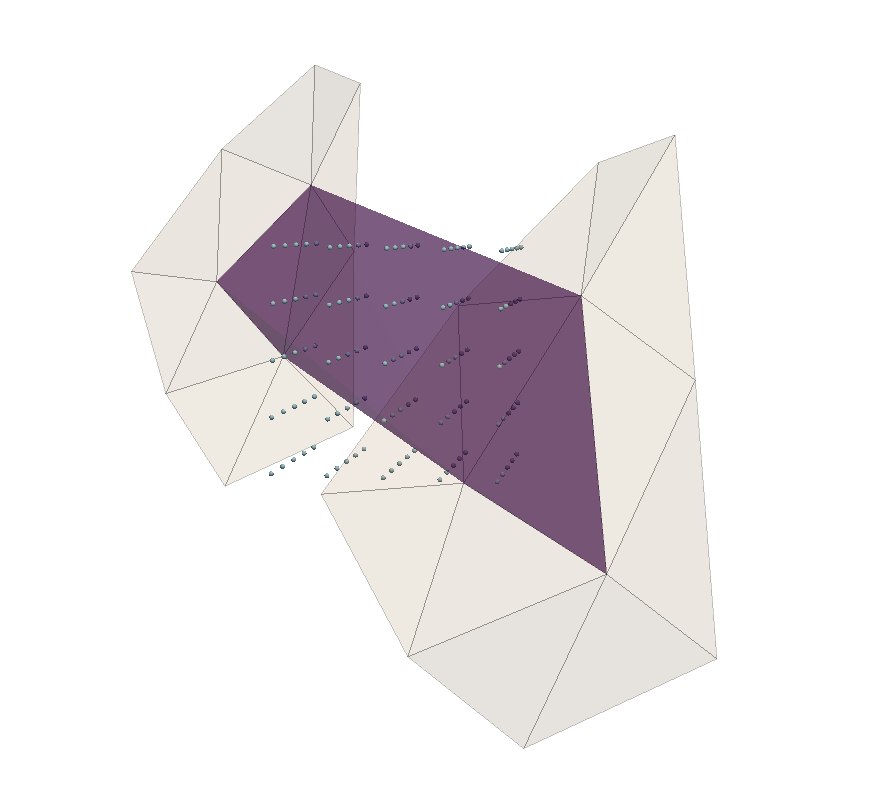
\includegraphics[width=0.45\textwidth]{prism1}}
\caption{Two alternative views of the triangular prism (purple) formed by connecting one pair of corresponding triangles on the inner and outer surfaces (grey) of the cortex. The subdivision into three tetrahedra is not shown. A $5^3$ grid of sample points are tested to determine the volume of intersection between the voxel and prism, which is recorded in the voxel-triangle matrix.} 
\label{prism}
\end{figure}

This approach is very similar to that of Toblerone's PV estimation algorithm from chapter \ref{tob_pv_chapter}, which uses convex hulls to determine the volume of intersection between a patch of surface and a voxel. There is however a subtle but important distinction. Toblerone's PV estimation estimates the total amount of cortical tissue per \textit{voxel}. This is a reduction operation that sums together all of the contributions of the surface primitives within a given voxel. By contrast, this process estimates the contributions of neighbourhood voxels per \textit{surface primitive}, which is the other way around and does not involve a reduction operation. 

\subsection{Points-triangle matrix}
The points triangle matrix records the area of each triangle on the cortical midsurface that `belongs' to its individual vertices (though vertices are now referred to as points to avoid re-using the letter $v$). These values are calculated using the Voronoi region approach, extended to arbitrary meshes by Meyer \textit{et al.} \cite{Meyer2003}, and are recorded in the matrix denoted $\mat{PT}$, sized (points x triangles). 

\begin{equation}
\mat{PT} = 
\begin{bmatrix}
pt_{11} & \ldots & pt_{1t} \\
\vdots & \ddots & \vdots \\
pt_{p1} & \ldots & pt_{pt}
\end{bmatrix}
\end{equation}

The element $pt_{pt}$ denotes the area of triangle $t$ that belongs to point $p$. Once again, this matrix is highly sparse as each point is associated to only a few triangles. 

\subsection{Forward projection}

\subsubsection{Volume to surface}
To form the volume to surface projection, the voxel-triangle matrix and point-triangle matrices are first normalised in a row or column-wise sense. This operation is denoted with the $\left\Vert \cdot \right\Vert_{row}$ operator defined below and rescales all rows or columns with non-zero sum such that they sum to unity. 

\begin{eqnarray}
\left\Vert \cdot \right\Vert_{row} &:& \mathrm{A}^{n \times m} \rightarrow \mathrm{A}^{n \times m} \nonumber \\
(\left\Vert \mathrm{A}^{n \times m} \right\Vert_{row})_{ij} &=&
\begin{cases}
a_{ij} / \sum^m_{k=0} a_{ik} & \text{if } \sum^m_{k=0} a_{ik} > 0 \\ 
0 & \text{if } \sum^m_{k=0} a_{ik} = 0 
\end{cases}
\end{eqnarray}

For the $\mat{VT}$ matrix, this is equivalent to ensuring that the sum of voxel weights for each triangle is unity, and for the $\mat{PT}$ matrix, that the sum of triangle areas for each point is unity. The effect of this is to turn these individual projections into weighted-averaging operations that preserve signal intensity. The overall projection is then defined by the multiplication

\begin{equation}
\mathrm{VS} = \left\Vert\mathrm{PT}\right\Vert_{row} \left\Vert \mathrm{VT} \right\Vert_{col}^T
\end{equation}

\subsubsection{Volume to hybrid}

In order to extend the forward projection into hybrid space, it is necessary to include the mapping between voxels and subcortical nodes (the $\mat{VS}$ matrix accounts only for cortical nodes). This is achieved by concatenating the $\mat{VS}$ matrix with the identity $\mat{I}_v$ matrix of size (number of voxels) to yield $\mat{VH}$, as illustrated in figure \ref{v2n_mat}. This implies a one-to-one mapping for all voxels to their hybrid space counterpart. 

\begin{equation}
\mathrm{VH} =  \begin{bmatrix}
    \begin{array}{c}
  \mathrm{VS}  \\
  \hline
  \mathrm{I}_v \\
    \end{array}
  \end{bmatrix}
\end{equation}

\subsubsection{Edge up-scaling}

Depending on the nature of the data that is to be projected, edge up-scaling is an optional extra step that can be incorporated into the forward projection. For signals that scale directly with the amount of tissue in a voxel, signal magnitude will be artificially low in any edge voxels that are less than 100\% brain (for example, those that contain some CSF which does not contribute any signal). In this case, it may be advantageous to up-scale the signal to account for the `lost' intensity. This is performed by calculating the voxel-wise brain PV (the sum of GM and WM PVs), taking the inverse of this quantity, and finally taking the outer product with the volume to surface projection matrix. The $\otimes$ operator denotes the outer product of a matrix and vector, in this case multiplying the \textit{j}th column of a matrix by the \textit{j}th value in a vector (referred to as `broadcasting' in NumPy or MATLAB). 

\begin{equation}
u_{i} = 
\begin{cases}
(\vec{pv}_{gm,i} + \vec{pv}_{wm,i})^{-1} & \text{if } \vec{pv}_{gm,i} + \vec{pv}_{wm,i} > 0 \\ 
0 & \text{if } \vec{pv}_{gm,i} + \vec{pv}_{wm,i} = 0 
\end{cases}
\end{equation}

\begin{equation}
\begin{aligned}
\otimes : \vec{b}^m, \mathrm{A}^{n \times m} \rightarrow \mathrm{A}^{n \times m} \\
(\vec{b} \otimes \mathrm{A})_{ij} = b_{j} a_{ij} 
\end{aligned}
\end{equation}

\begin{equation}
\mathrm{VH}_{edge} =  \begin{bmatrix}
    \begin{array}{c}
  \vec{u} \otimes \mathrm{VS}  \\
  \hline
  \vec{u} \otimes \mathrm{I}_v \\
    \end{array}
  \end{bmatrix}
\end{equation}

The purpose of this step is to perform a very simple correction for signal lost due to PVE. It is however \textit{not} the same as performing PVEc: that operation attempts to separate out different signal contributions, whereas this operation up-scales the aggregate signal (therefore maintaining the ratio of signal contributions equal). An example of where this step could be applied is projection of ASL or BOLD data (signal scales with tissue PV); an example of where it would not be appropriate is projection of a timing volume (such as voxel-wise inversion time data, which are independent of tissue PV). 

\subsection{Reverse projection}

\subsubsection{Surface to volume}
To form the surface to volume projection, the voxel-triangle and point-triangle matrices are normalised in the opposite sense to before. For the voxel-triangle, this is equivalent to ensuring that the sum of triangle weights for each voxel is unity, and for the point-triangle matrix, that the sum of vertex areas for each triangle is unity. The surface to volume projection is then defined by the multiplication of the two.  

\begin{equation}
\mathrm{SV} =  \left\Vert \mat{VT} \right\Vert_{row} \left\Vert \mat{PT} \right\Vert_{col}^T
\end{equation}

\subsubsection{Hybrid to volume}

In order to form the reverse projection from hybrid space, PVE must be recreated. This follows from the fact that nodes in hybrid space enforce the separation of signals from different tissues. Each row of the hybrid to volume projection matrix corresponds to a voxel, and the column values record the weights in which both cortical and subcortical nodes contribute to that voxel. A set of voxel-wise GM and WM PV estimates are then used to scale the overall contribution of cortical and subcortical nodes within each voxel\footnote{Note the double-scaling here, which reflects the slightly different types PVE at work. Firstly, there is the question of determining the relative contributions of the different cortical nodes within the voxel; secondly, there is the question of determining the relative contributions of the cortical versus subcortical components of signal.}. In particular, each row of the surface-to-volume matrix is scaled by the GM PV of the corresponding voxel, and each row of the identity by the WM PV of the corresponding voxel. 

\begin{equation}
\mathrm{HV} = [\ \vec{pv}_{gm} \otimes \mat{SV} \ | \ \vec{pv}_{wm} \otimes \mat{I}_v \ ]
\end{equation}

\subsubsection{Edge down-scaling}

Edge down-scaling may optionally be applied for the reverse projection depending on the nature of the data in question. The same principles as for the forward case apply: if the signal is expected to scale with tissue PV, then edge scaling reduces the projected signal in voxels that are less than 100\% brain. In this situation, there is a subtle distinction between PVE caused by \textit{mixed} signal and PVE caused by \textit{missing} signal, though both originate in the same manner (the presence, or absence, of multiple tissues in a voxel). Edge down-scaling is achieved by calculating the total brain PV $\vec{b}$ in each voxel and then taking the outer product with the relevant projection matrix. 

\begin{equation}
\vec{b} = \vec{pv}_{gm} + \vec{pv}_{wm}
\end{equation}
\begin{equation}
\mathrm{HV}_{edge} = \vec{b} \otimes \mat{HV}
\end{equation}

\begin{figure}[H]
\centering
\subcaptionbox{\label{v2n_mat}}[0.45\textwidth]
{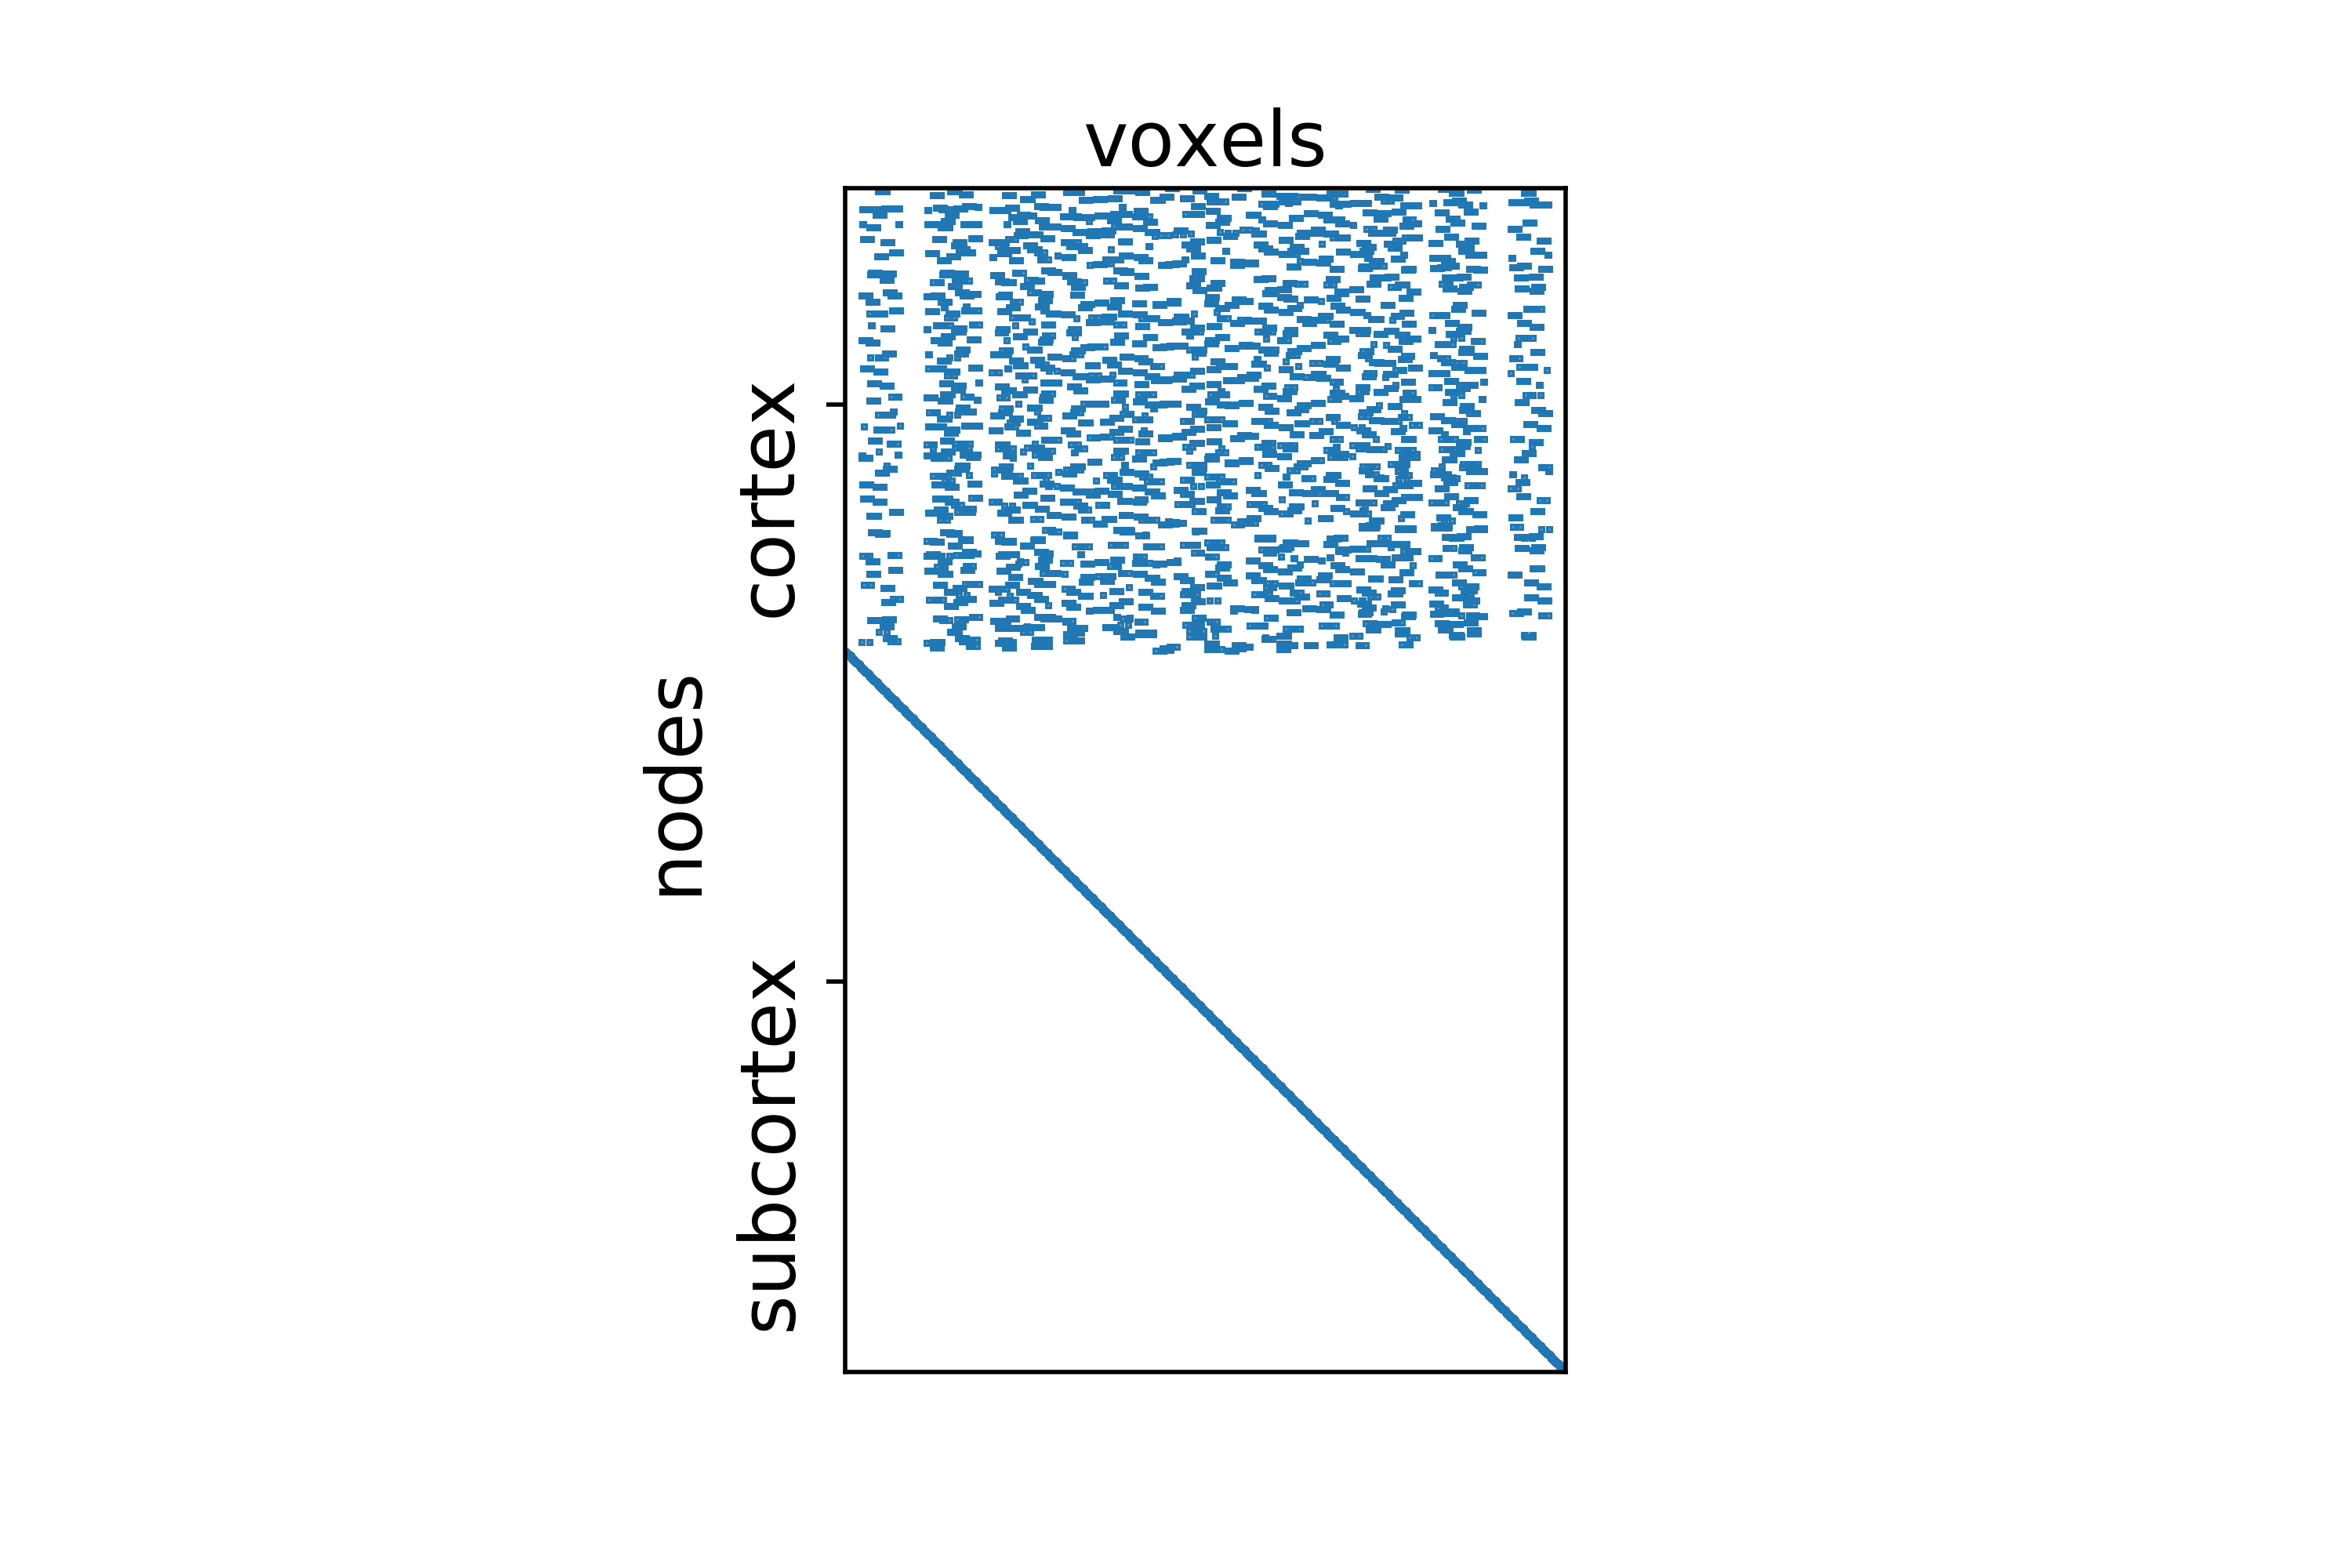
\includegraphics[width=0.45\textwidth]{v2n}}
\subcaptionbox{\label{n2v_mat}}[0.45\textwidth]
{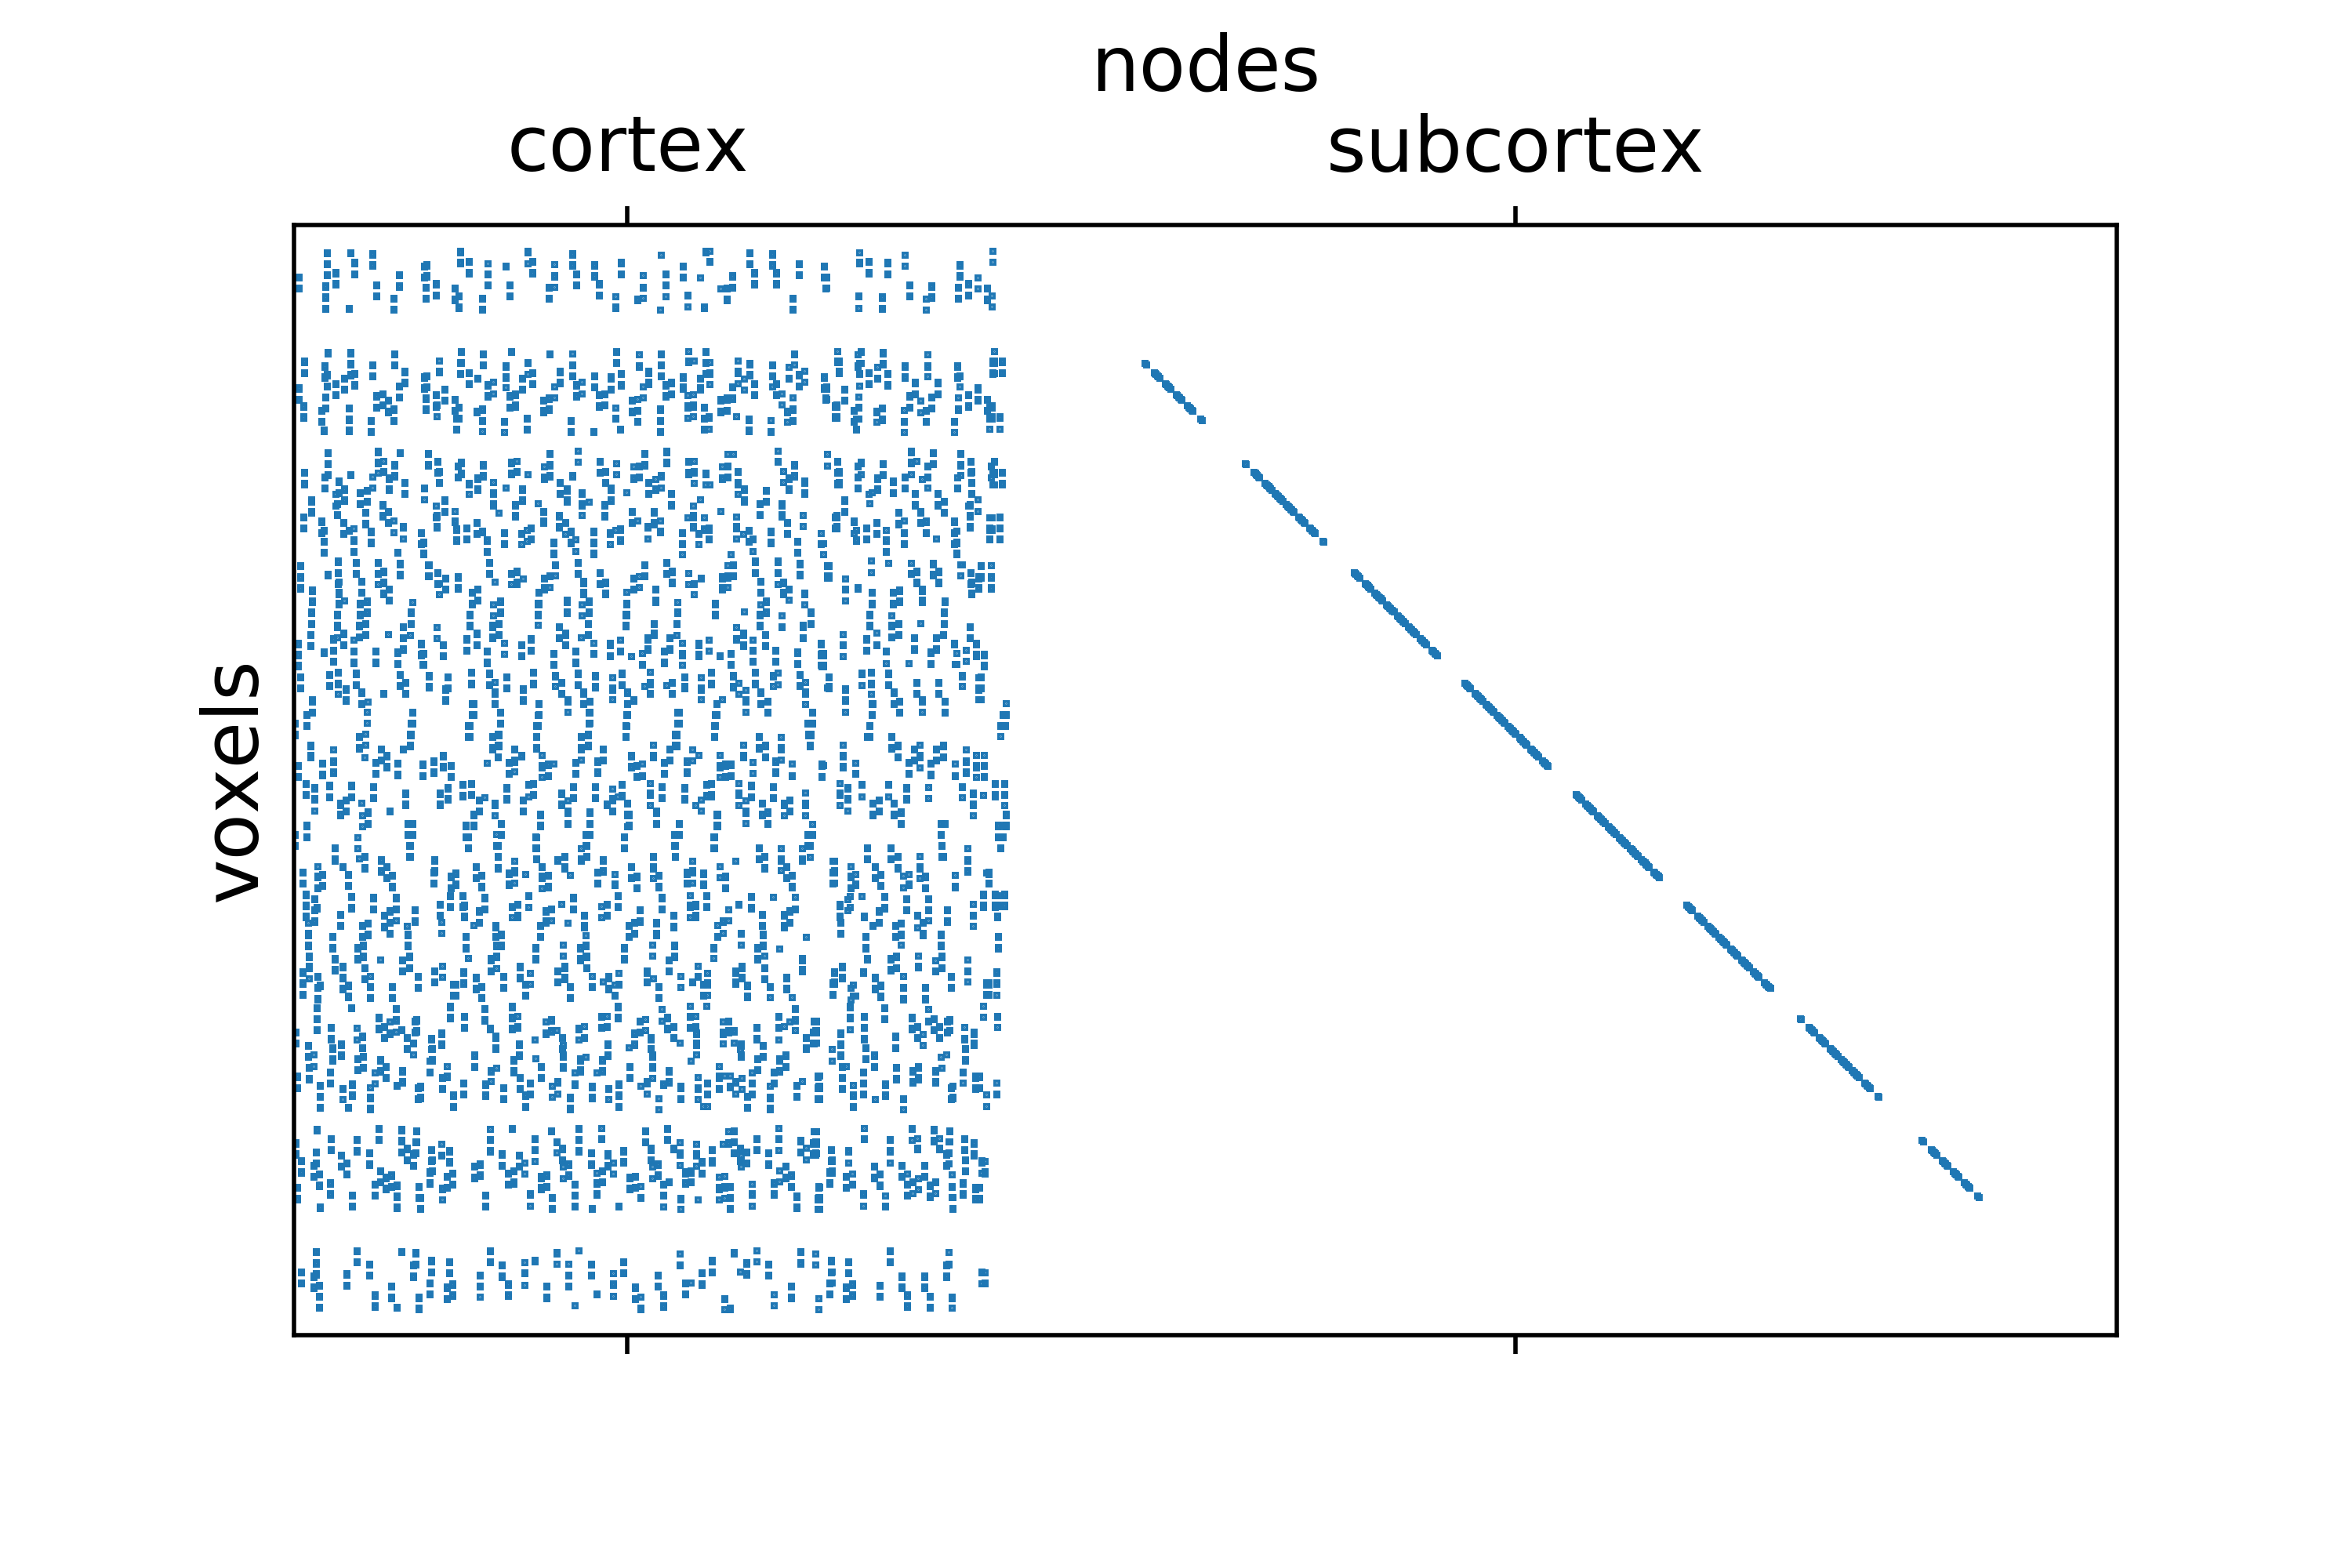
\includegraphics[width=0.45\textwidth]{n2v}}
\caption{Sparsity structure of the (a) volume to hybrid without edge up-scaling and (b) hybrid to volume with edge down-scaling projection matrices. The portions of each corresponding to cortex and subcortex are labelled.} 
\label{sparsity}
\end{figure}

All of the projection matrices here described are highly sparse (illustrated in figure \ref{sparsity}). Accordingly, the implementation of these within the Toblerone software package makes extensive use of the NumPy and SciPy sparse matrix packages \cite{Walt2011, Virtanen2020}.


\section{Methods}
Evaluation of Toblerone's projection has been performed using cortical surfaces drawn from the HCP database \cite{HCP_data, Glasser2013} and simulated physiological data. Left cortical hemispheres at 32k mesh resolution for 45 subjects from the test-retest dataset were used. A 2.2mm isotropic voxel grid was used to approximate physiological imaging resoltion for all subjects. The HCP's RC method was used as a comparator. By using the \textit{-output-weights-text} option with the \textit{wb\_command -volume-to-surface-mapping} tool, the projection weights used by the RC method were saved to file and the corresponding matrices reconstructed. Comparisons between Toblerone and RC were performed using a paired $t$-test with significance threshold p $<$ 0.001. 

Although Toblerone and the RC method allow both the forward and reverse projections to be constructed directly, these matrices are not true inverses of each other. This arises due to the non-square dimensionality of the system: at typical functional resolution, there are multiple surface vertices present in each voxel and so the system is over-determined in one direction and under-determined in the other. Previous work in the field (notably, the inverse surface approach of \cite{Lonjaret2017}) has formulated the over-determined system directly (surface to volume) and then attempted to invert it to obtain a volume to surface projection. Accordingly, such an approach was used as an extra comparator for both Toblerone and RC. The least-squares QR solver (lsQR, \cite{10.1145/355984.355989}) implemented in SciPy's sparse linear algebra package is able to solve both under- and over-determined matrix equations of the form $\mathrm{A}\vec{x} = \vec{b}$ given the sparse matrix $\mat{A}$ and a vector of values $\vec{b}$. lsQR does not attempt to find the inverse matrix $\mat{A}^{-1}$ explicitly but instead seeks to approximate the solution via QR factorisation. Because of this, it is not possible to use lsQR to find a reverse projection matrix in the general case; it can only be used in specific cases to obtain $\vec{x}$ given a vector $\vec{b}$ of forward-projected values. 

\section{Datasets}
\subsection{Local signal tests}
The objective of this experiment was to investigate the localisation and intensity of signals following projection. Due to the lack of a ground truth projection method to use as a gold standard, round-trip projections were instead performed to assess the self-consistency of each method. A ground truth signal peak (approximating an activation) was generated for each subject by selecting a random vertex $N$ from areas of cortex with local thickness greater than 1mm (to exclude very high levels of PVE) and finding its connected neighbours (denoted $N_1$ and $N_2$ for the first- and second-order neighbourhoods respectively). These vertices were then assigned the values 1, 0.8 and 0.6 for $N$, $N_1$ and $N_2$ respectively. All other vertices had zero signal. An example activation is shown in figure \ref{activation_example}. 

\begin{figure}
\centering
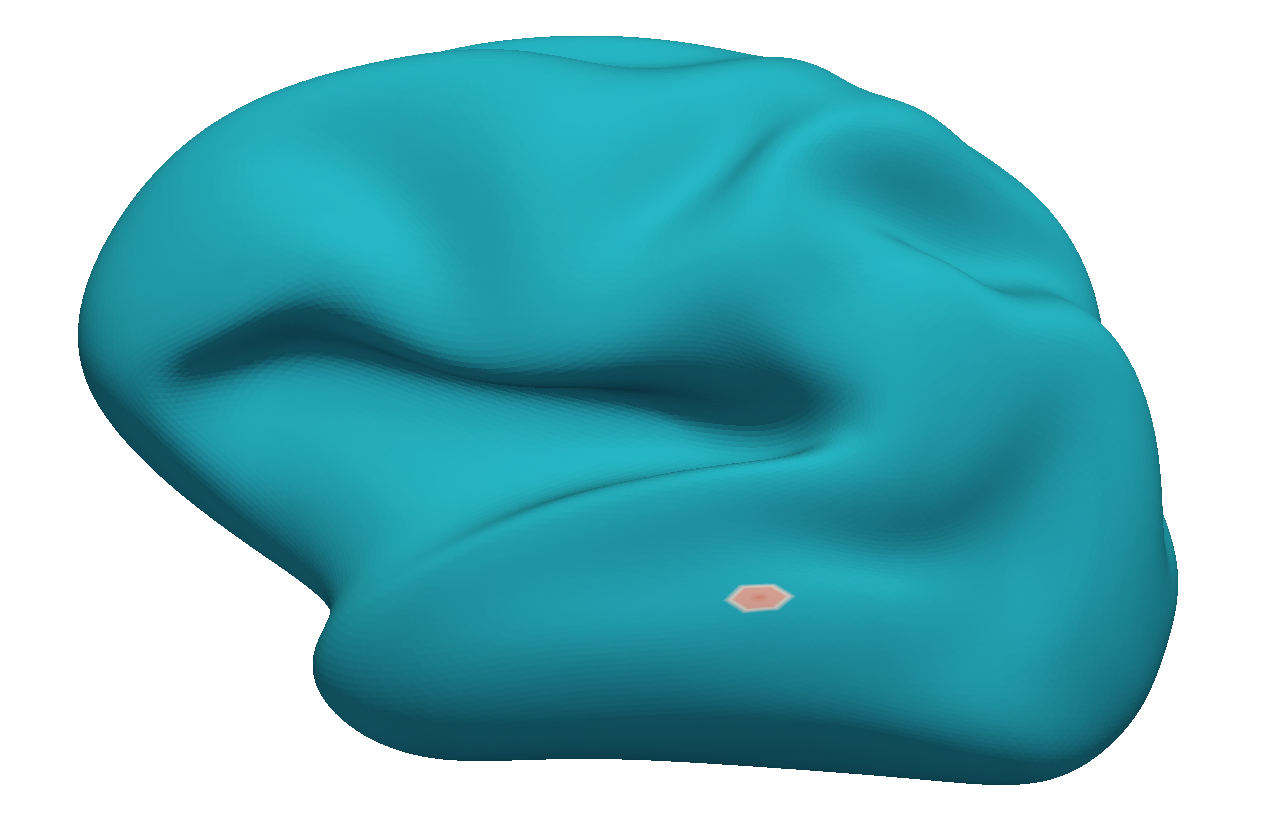
\includegraphics[width=0.6\textwidth]{activation}
\caption{Example activation for subject 103818 from the HCP dataset, left cortical hemisphere. A random vertex has value 1; the 1-neighbours have value 0.8; and the 2-neighbours have value 0.6. All other values are zero. Note that the signal peak was defined on the cortical midsurface but is illustrated here on the inflated surface.}
\label{activation_example} 
\end{figure}

The ground truth surface activation was projected into the 2.2mm isotropic voxel grid, and then back onto the surface, using both Toblerone's surface-volume projection and the RC method. Peak signal intensity in both volume space (after one projection) and surface space (after both projections) was recorded. The desired outcome of this analysis is that an activation should map to a maximal voxel signal in volume space; when the projection is reversed, the original signal value should be recovered (in the ideal case). Spreading out of signal on the surface was also investigated using the count ratio of non-zero vertices between the twice-projected data and ground truth. In the ideal case this ratio would be unity as the round-trip of projection would not lead to smoothing of signal (a consequence of the averaging that is incorporated into both projection methods). 

\subsection{Global signal tests}
The objective of this experiment was to investigate the fidelity with which globally distributed signals are projected. Round-trip projections were performed in both a volume-surface-volume and surface-volume-surface sense; a schematic for the latter is shown in figure \ref{SVS_schematic}. Three variants of Toblerone's projection were investigated, as shown in table \ref{projection_variants}. All variants incorporated edge down-scaling in the surface (or hybrid) to volume direction, which is equivalent to the behaviour of RC. By contrast, RC does not provide edge up-scaling in the volume to surface direction. Note that in the case of hybrid projection, the corresponding data by definition contains both cortical and subcortical signal. 

\begin{table}[H]
\centering
\def\arraystretch{1.5}
\begin{tabular}{p{3cm}|p{11cm}}
\textit{variant} & \textit{meaning}                                                                                                                                             \\ \hline
surface          & Volume-surface projection, directly comparable to RC. Data contains only cortical signal.                                                                                                         \\
surface + edge & Volume-surface projection, with edge up-scaling in the volume to surface direction. Data contains only cortical signal. 
\\
hybrid + edge  & Volume-hybrid projection, with edge up-scaling in the volume to hybrid direction. Data contains cortical and subcortical signal.                                                                                \end{tabular}
\caption{The different variants of Toblerone's projection investigated. The hybrid variant requires data that contains both cortical and subcortical signal.}
\label{projection_variants}
\end{table}

For each variant of projection, three signal distributions were tested: flat, sinusoidally varying and randomly distributed, the properties of which are given in table \ref{signaltable}. This resulted in nine combinations of (projection variant, signal distribution) pairs. 

\begin{table}[H]
\centering
\def\arraystretch{1.5}
\newcommand{\wrap}[1]{\parbox{\linewidth}{\vspace{1.5mm}#1\vspace{1mm}}}
\begin{tabular}{p{4cm}|p{1.5cm}p{5cm}p{3cm}}
& \textit{flat}  & \textit{sine} & \textit{random} \\ \hline
cortical GM ($\vec{f}_{gm}$) & 60 & \wrap{60 $\pm$ 18 \\ peak-peak separation \mytilde36mm} & 60 + 10 $N$(0,4) \\
subcortical WM ($\vec{f}_{wm}$) & 20 & \wrap{20 $\pm$ 6 \\ peak-peak separation \mytilde36mm} & 20 + 5 $N$(0,2) \\
\end{tabular}
\caption{Signal distribution properties. The cortex was assumed to be GM and all other tissue WM.}
\label{signaltable}
\end{table}


\begin{figure}[H]
\centering
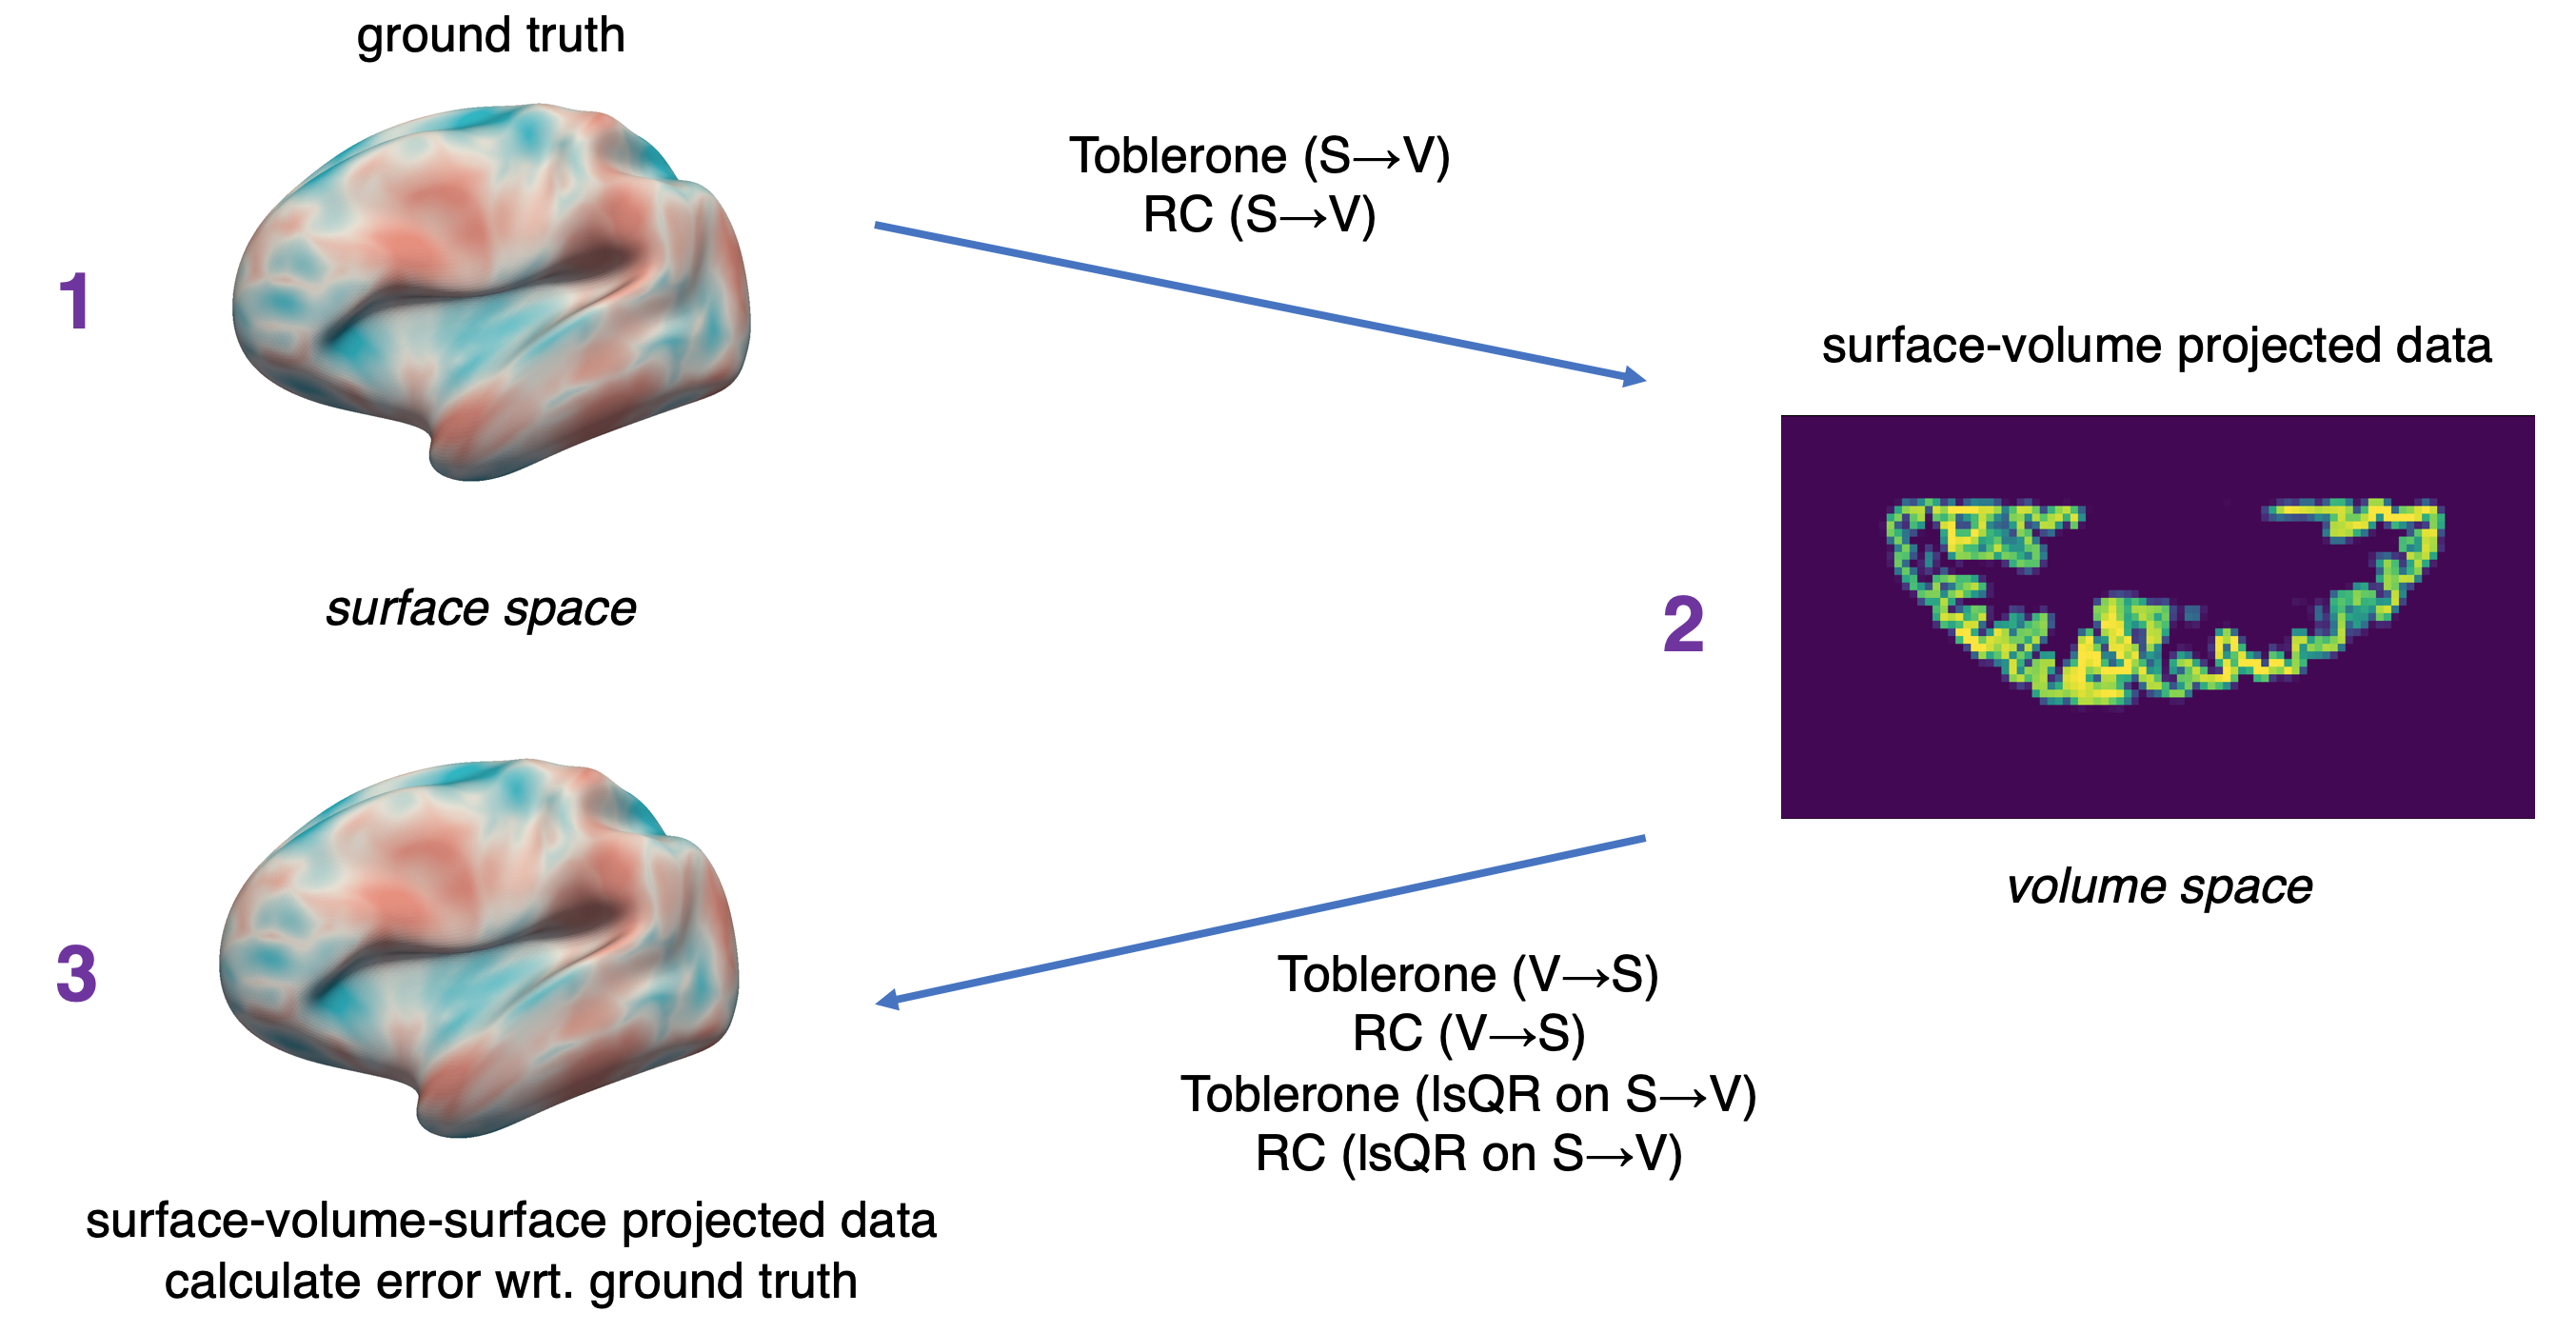
\includegraphics[width=\textwidth]{SVS_schematic}
\caption{Schematic of the surface-volume-surface global signal projection test. Two forward projections are used for surface-volume and four reverse projections are used (each method's self-inverse, alongside the lsQR-inverse of each). The volume-surface-volume test had a similar layout, with the surface and volume spaces swapped.}
\label{SVS_schematic} 
\end{figure}

\begin{figure}[H]
\centering
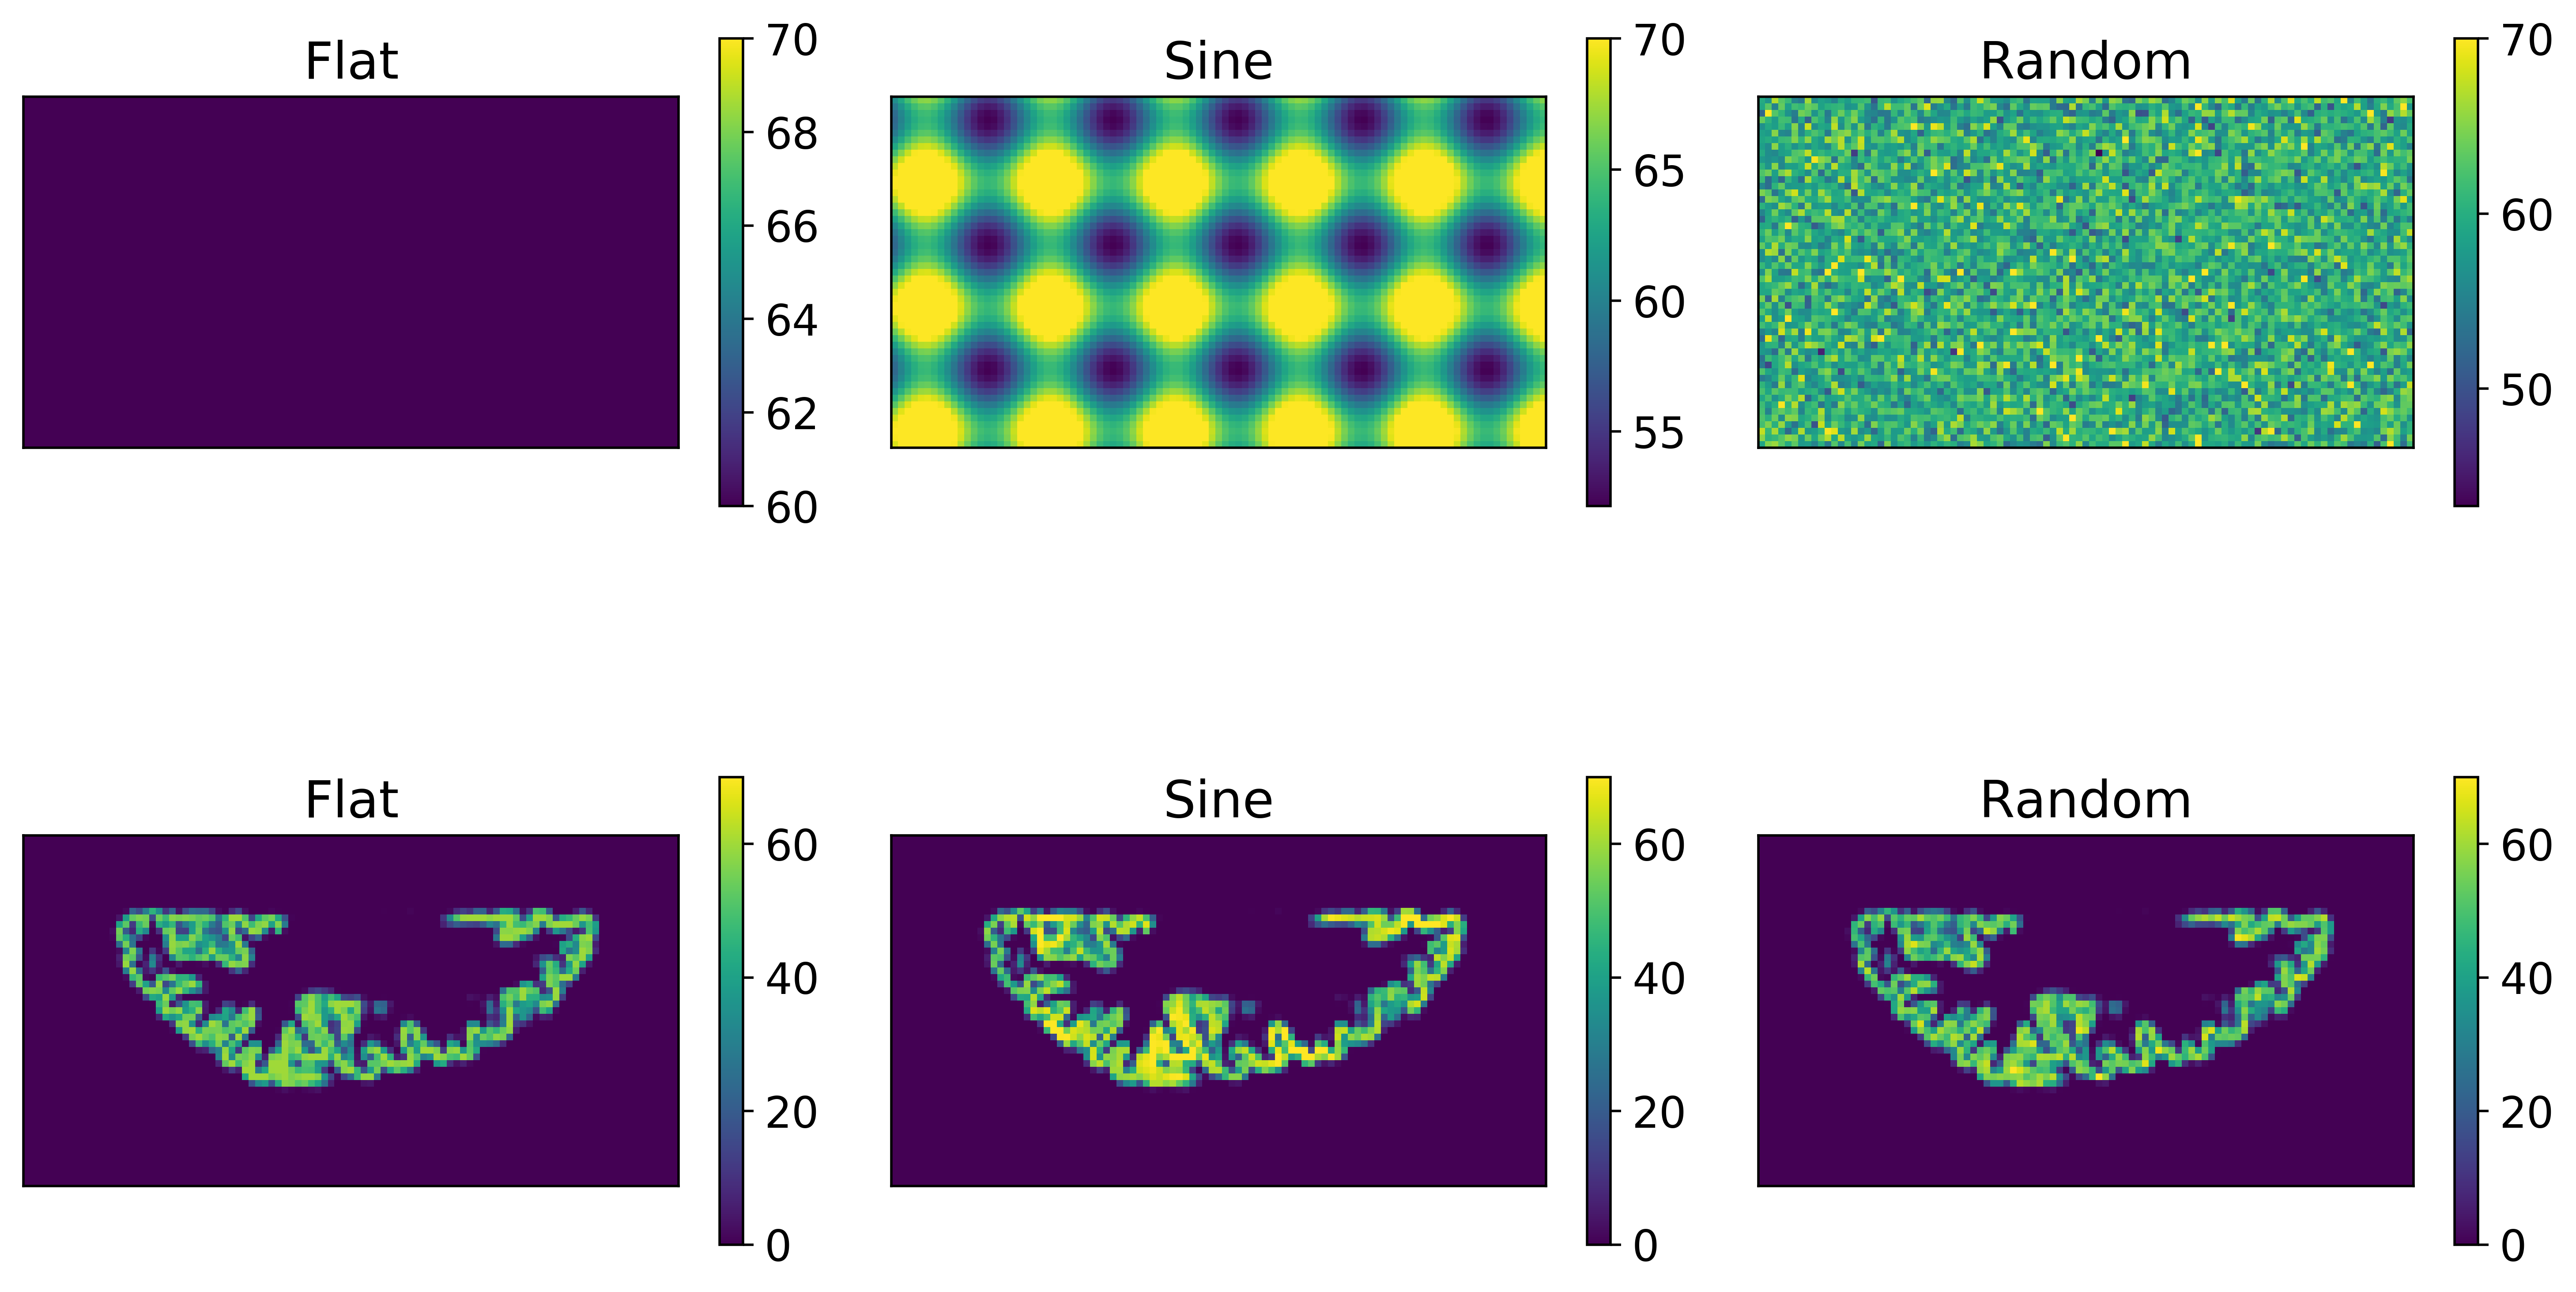
\includegraphics[width=\textwidth]{vtruths}
\caption{Volumetric ground truths for subject 103818 of the HCP dataset. Top row: signal distribution fields (GM). Bottom row: volumetric data produced by multiplying GM PV maps for this subject with each field.}
\label{vol_truth} 
\end{figure}

Ground truth volume data were produced by evaluating volumetric fields of values for each of the signal distributions (illustrated in the top row of figure \ref{vol_truth}) and then modulating these using subject-specific PV maps (produced by Toblerone's PV estimation algorithm). This is represented by the following equation, where $\vec{g}_v$ denotes volumetric ground truth, $\vec{f}_{gm}$ denotes the vector of field values (flat, sine, random) for GM and $\vec{pv}_{gm}$ the vector of GM PV estimates.

\begin{equation}
\vec{g}_v = \vec{f}_{gm} \cdot \vec{pv}_{gm} + \vec{f}_{wm} \cdot \vec{pv}_{wm}
\end{equation}

In order to produce cortex-only signals (i.e, neglecting subcortical signal contributions), the WM portion of this equation was omitted. Example volumetric ground truths for a single subject are given in the bottom row of figure \ref{vol_truth}. 

Ground truth surface data was produced by interpolating from the respective field values onto the vertices of each subject's cortical midsurface using trilinear interpolation. An example surface ground truth is given in figure \ref{surf_truth}. For projection to and from hybrid space, it is necessary to provide signal values for the nodes that represent the subcortex. This was achieved by the concatenating the volumetric WM signal for each field onto the vector of interpolated surface values, where $S(\vec{f}_{gm})$ denotes the interpolated field values $\vec{f}_{gm}$ on the surface, and $\vec{f}_{wm} \cdot \vec{pv}_{wm}$ represents the volumetric signal for the subcortex. This step is justified on the basis that the projection assumes subcortical nodes to have a one-to-one mapping with their corresponding voxels. As the RC method has no concept of hybrid space, in this comparison it operated only on the surface component of the data. 

\begin{equation}
\vec{g}_s =  [\ S(\vec{f}_{gm}) \ | \ \vec{f}_{wm} \cdot \vec{pv}_{wm} \  ]
\end{equation}

\begin{figure}
\centering
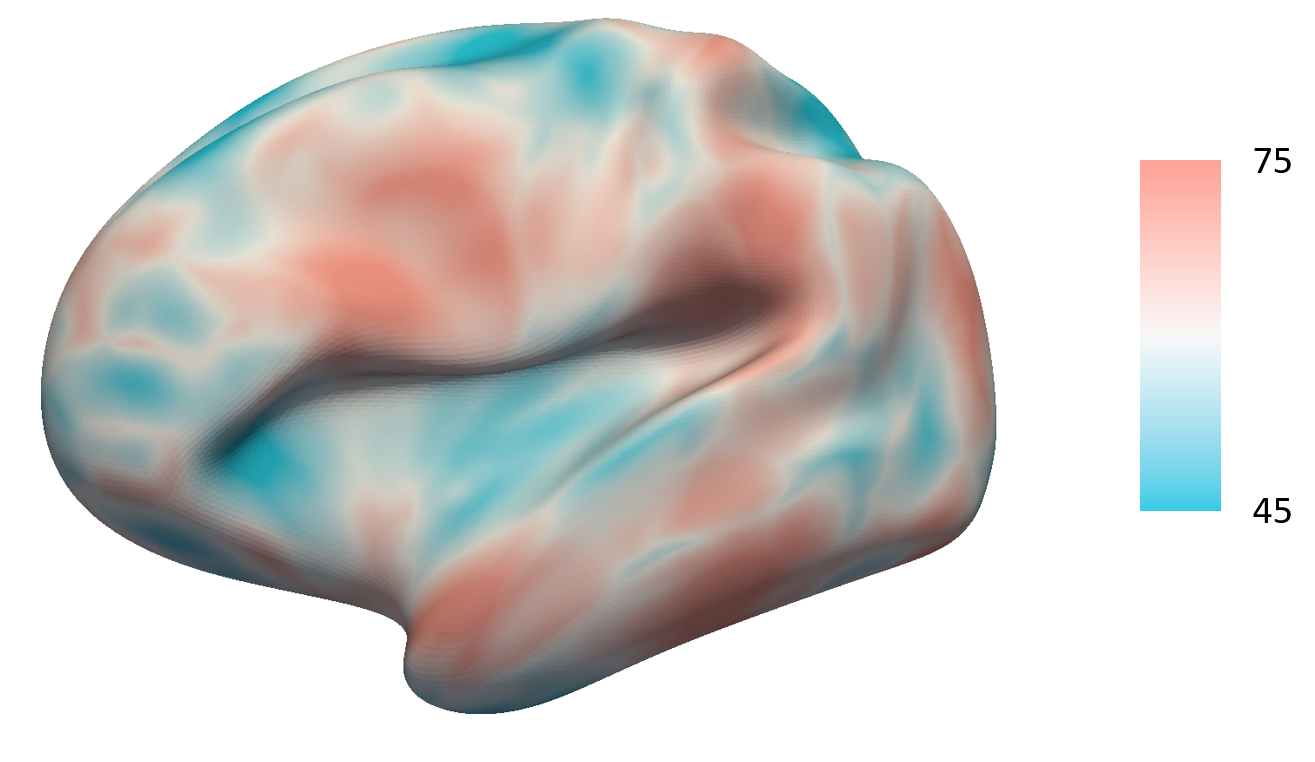
\includegraphics[width=0.7\textwidth]{struth}
\caption{Sinusoidally varying surface ground truth for subject 103818 of the HCP dataset (plotted on inflated surface).}
\label{surf_truth} 
\end{figure}

The metrics of interest for this experiment were global error and minimum/maximum signal intensity. Global error was measured using the RMS of differences, either measured in voxel-wise or in a vertex-wise manner. Volumetric projected output was masked to consider only voxels intersecting the cortex (defined by $\vec{pv}_{gm} >$ 0). Surface projected output was masked to consider only vertices with a cortical thickness greater than 1mm (avoiding excessive signal loss for all methods due to very high PVE in the surface-volume direction). Maximum signal intensity was measured as a fraction of the ground truth maximum value. In the ideal case, the round-trip projection would preserve signal intensity, but in practice signal is irreversibly lost due to PVE. Finally, the minimum value following each projection was recorded; in the ideal case, this should always be zero as no negative values were present in the ground truth data. Minimum and maximum projected values are indicative of the numerical stability of each projection method. 

\section{Results}

\subsection{Local signal tests}

\begin{figure}[H]
\centering
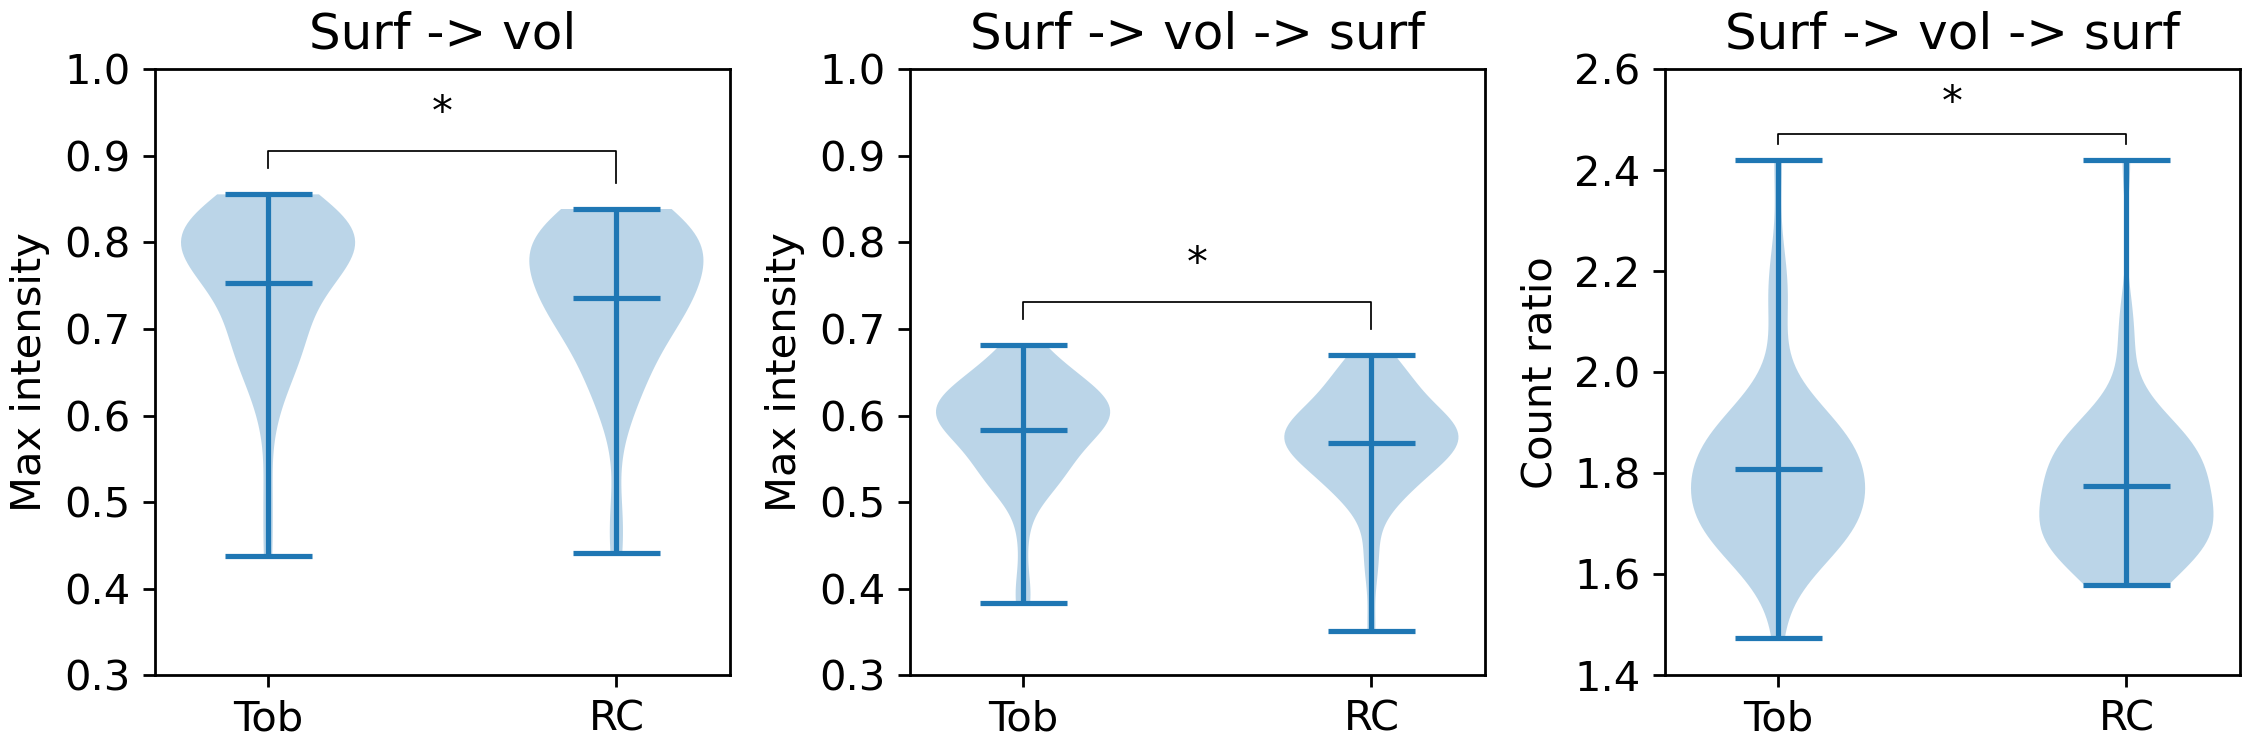
\includegraphics[width=\textwidth]{activation_results}
\caption{Local signal projection results. Left: peak voxel signal for each method. Centre: peak surface signal for each method (projected from volume), Right: ratio of non-zero vertices compared to ground truth. The means of each distribution are denoted with a central horizontal line for clarity. * denotes a paired $t$-test result with $p\leq $ 0.001.}
\label{local_results} 
\end{figure}

Figure \ref{local_results} shows the results of the local signal projection test. The leftmost plot shows peak voxel signal following surface-volume projection. The centre plot shows peak surface signal following surface-volume-surface projection. The rightmost plot shows the ratio of surface vertices that are activated following the second projection as a ratio of the ground truth value. In both volume and surface spaces, projection with Toblerone led to marginally higher peak signals compared to RC. Both methods displayed spreading out of signal across the surface, as evidenced by the count ratio $>$ 1, and Toblerone demonstrated marginally higher variability in this metric across subjects. All comparisons between Toblerone and RC met the significance threshold. 

\subsection{Global signal tests}

\begin{figure}[H]
\centering
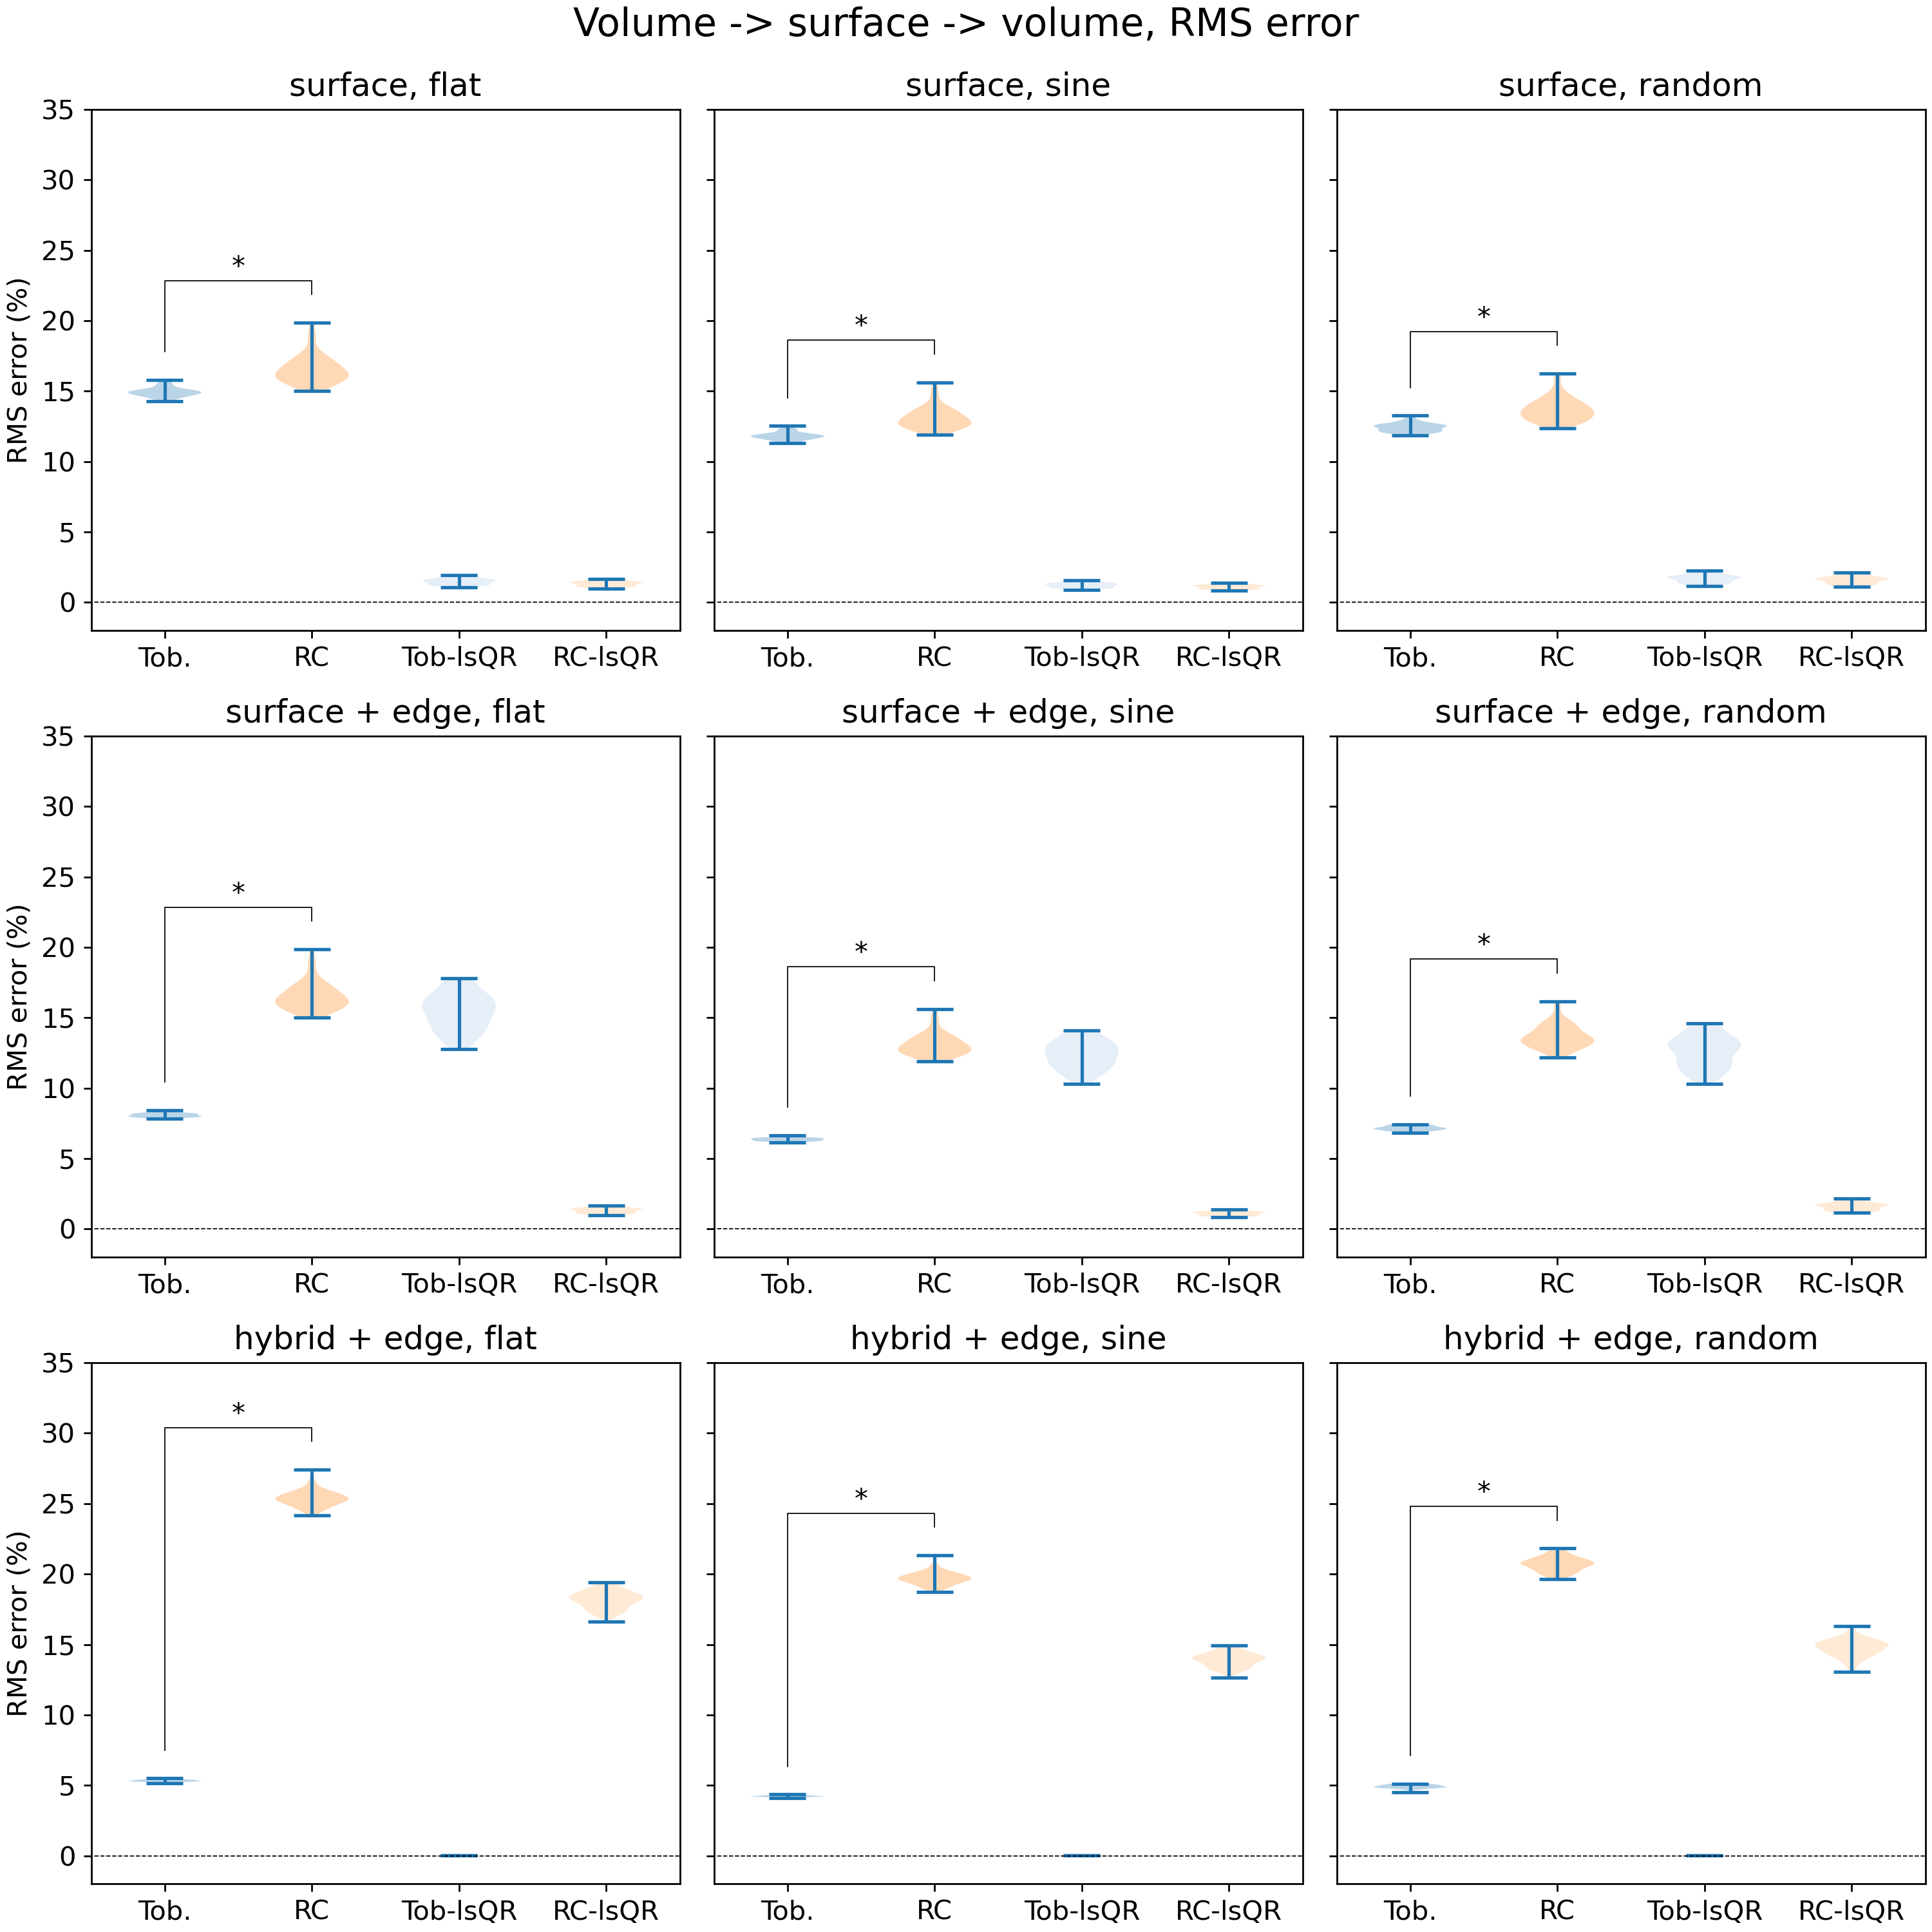
\includegraphics[width=\textwidth]{VSV_violins}
\caption{RMS error, volume-surface-volume projection. Errors for Toblerone's surface projection were somewhat lower than RC; when using edge scaling and/or the hybrid projection further significant reductions were observed. lsQR returned extremely low errors. * denotes a paired $t$-test result with $p\leq $ 0.001.}
\label{VSV_rms} 
\end{figure}

Figure \ref{VSV_rms} shows RMS voxel error for the volume-surface-volume global signal projection test. The errors for Toblerone's surface projection were somewhat lower than those of RC in all three signal distributions (flat, sine, random). With Toblerone's hybrid projection, further reductions in error were observed. The largest differences arose in the hybrid projection (RMS error of around 20\% for RC and around 5\% for Toblerone). The lsQR methods returned low errors (in many cases the error being essentially zero). All comparisons  between Toblerone and RC met the significance threshold. 

\begin{figure}[H]
\centering
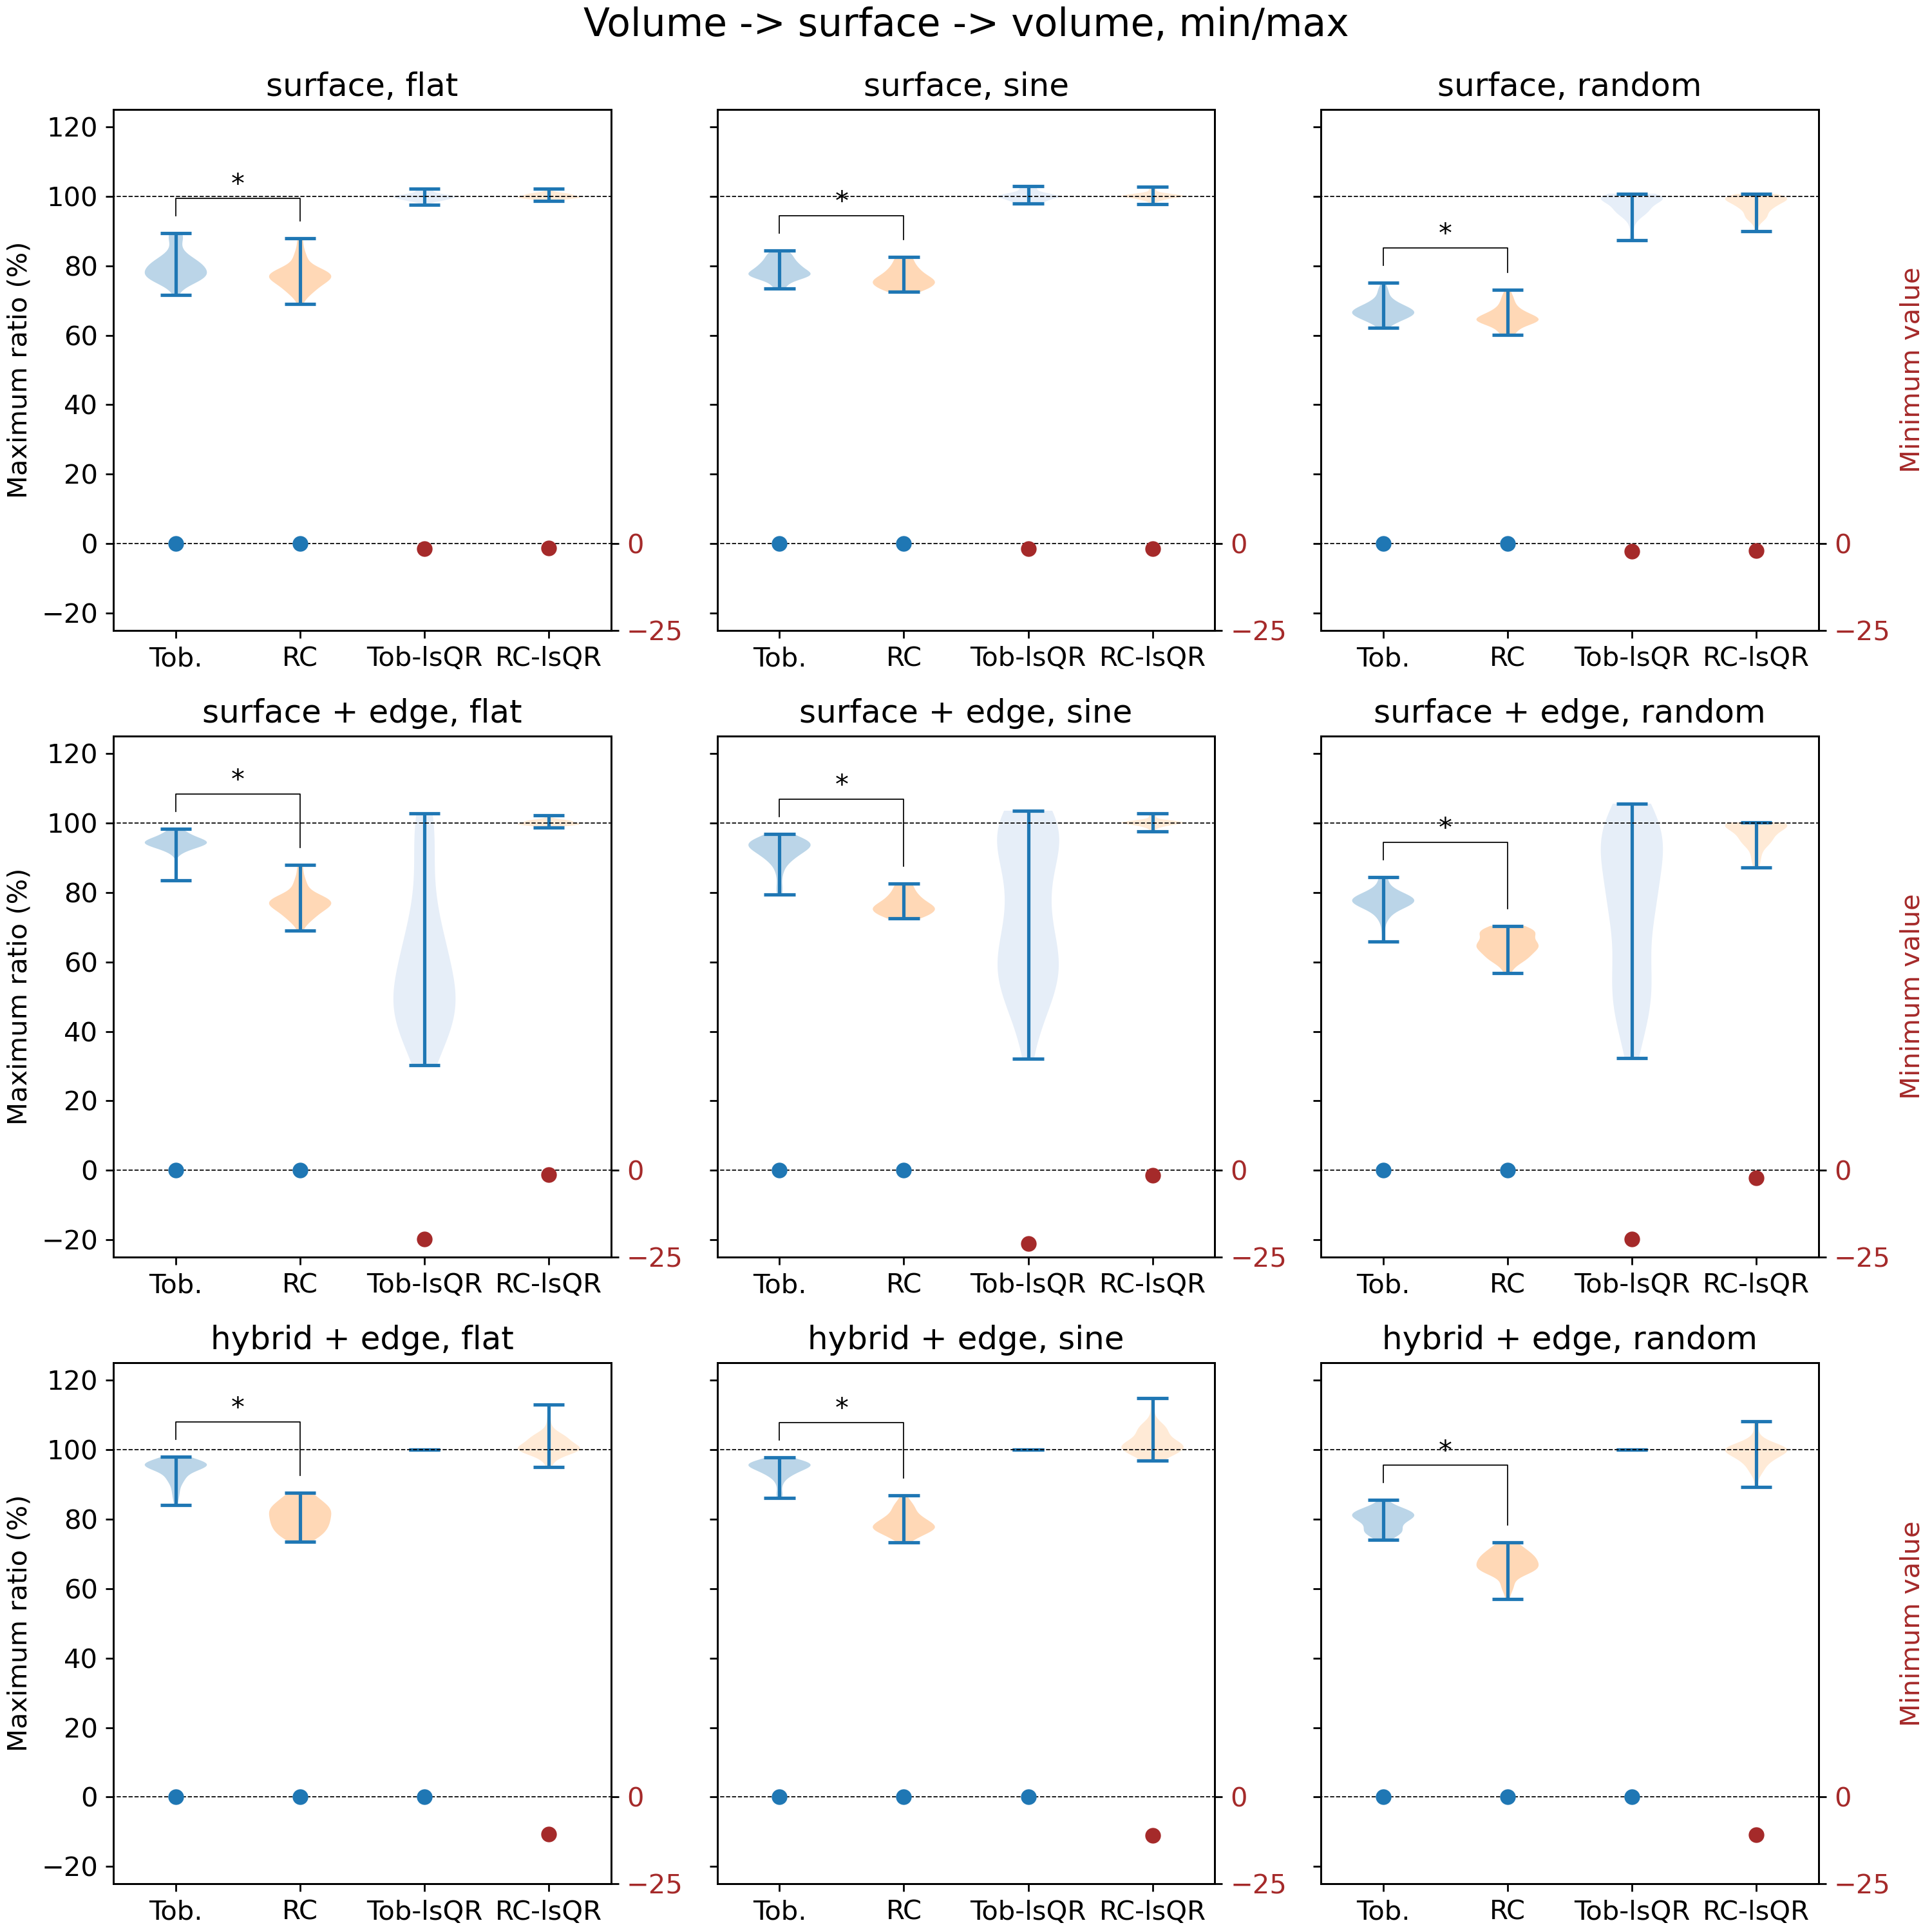
\includegraphics[width=\textwidth]{VSV_minmax}
\caption{Maximum and minimum values, volume-surface-volume projection. Toblerone's surface projection performed similarly to the RC method in preserving signal intensity (both methods around 80\%). Signal intensity increased when using edge scaling and/or the hybrid projection. lsQR methods occasionally returned values above 100\% or below zero. * denotes a paired $t$-test result with $p\leq $ 0.001.}
\label{VSV_minmax} 
\end{figure}

Figure \ref{VSV_minmax} shows maximum and minimum values for the volume-surface-volume projection test. Looking at the left hand scale on each plot, Toblerone's surface projection returned similar maximum signal intensities as RC. With the use of edge scaling, and the hybrid projection, higher maximum signal intensities were observed (around 95\% in the hybrid sine case, for example). The lsQR methods were able to almost perfectly preserve signal in most cases, though in some examples the signal overshot to around 110\% of reference value. The right hand scale of each plot shows mean minimum signal value for each method, with points in red denoting negative values. Whilst the minimum for the Toblerone and RC methods always remained at zero, for the lsQR methods it was occasionally negative (for example, around -15 for the RC-lsQR method, hybrid data, random distribution). All comparisons  between Toblerone and RC met the significance threshold. 

\begin{figure}[H]
\centering
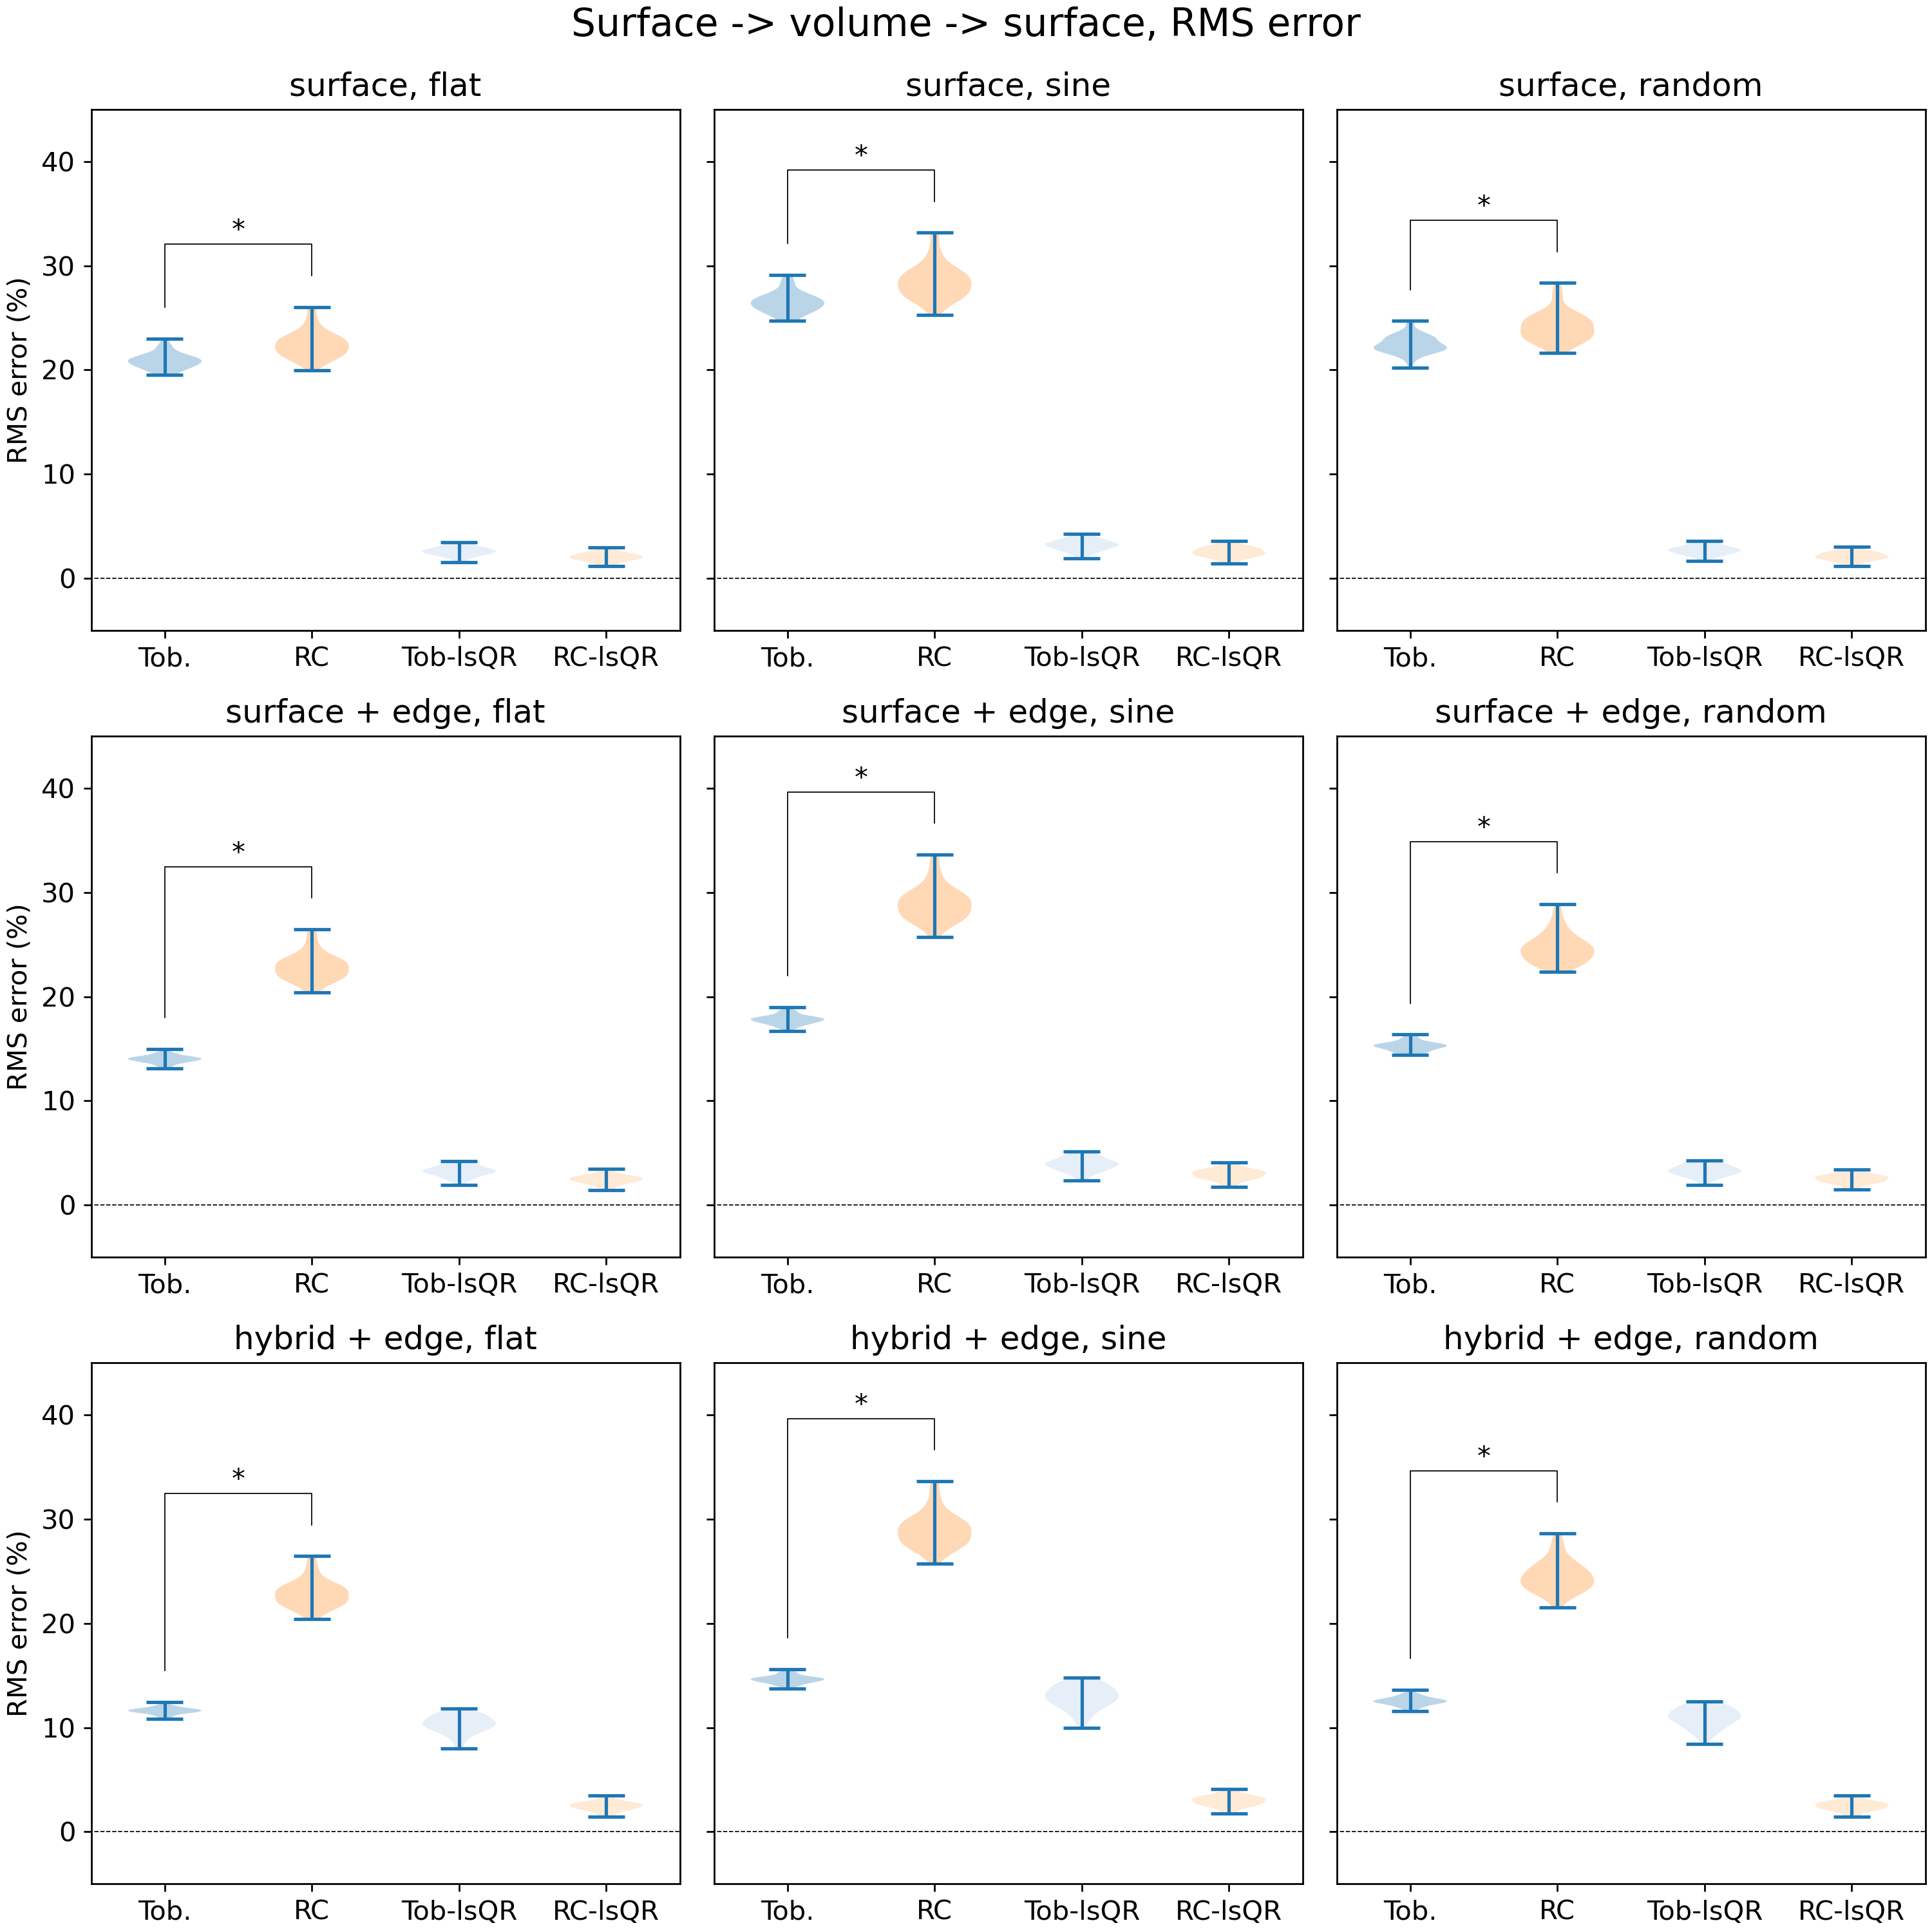
\includegraphics[width=\textwidth]{SVS_violins}
\caption{RMS error, surface-volume-surface projection. Surface projection with Toblerone produced marginally smaller errors than RC; with edge scaling and hybrid projection, error was further reduced. The lsQR method performed better with Toblerone's surface projection than the hybrid projection. * denotes a paired $t$-test result with $p\leq $ 0.001.}
\label{SVS_rms} 
\end{figure}

Figure \ref{SVS_rms} shows RMS error for the surface-volume-surface projection test. Toblerone's surface projection produced marginally lower errors than RC, and with the introduction of edge scaling and the hybrid projection, error was further reduced (from around 25\% to around 15\% in all three signal distributions). The lsQR methods again produced lower RMS errors overall, though they did not produce errors as low as they did on the volume-surface-volume test and the margin between Toblerone's hybrid projection and the lsQR equivalent was small (around 5\% at most). All comparisons  between Toblerone and RC met the significance threshold. 

\begin{figure}[H]
\centering
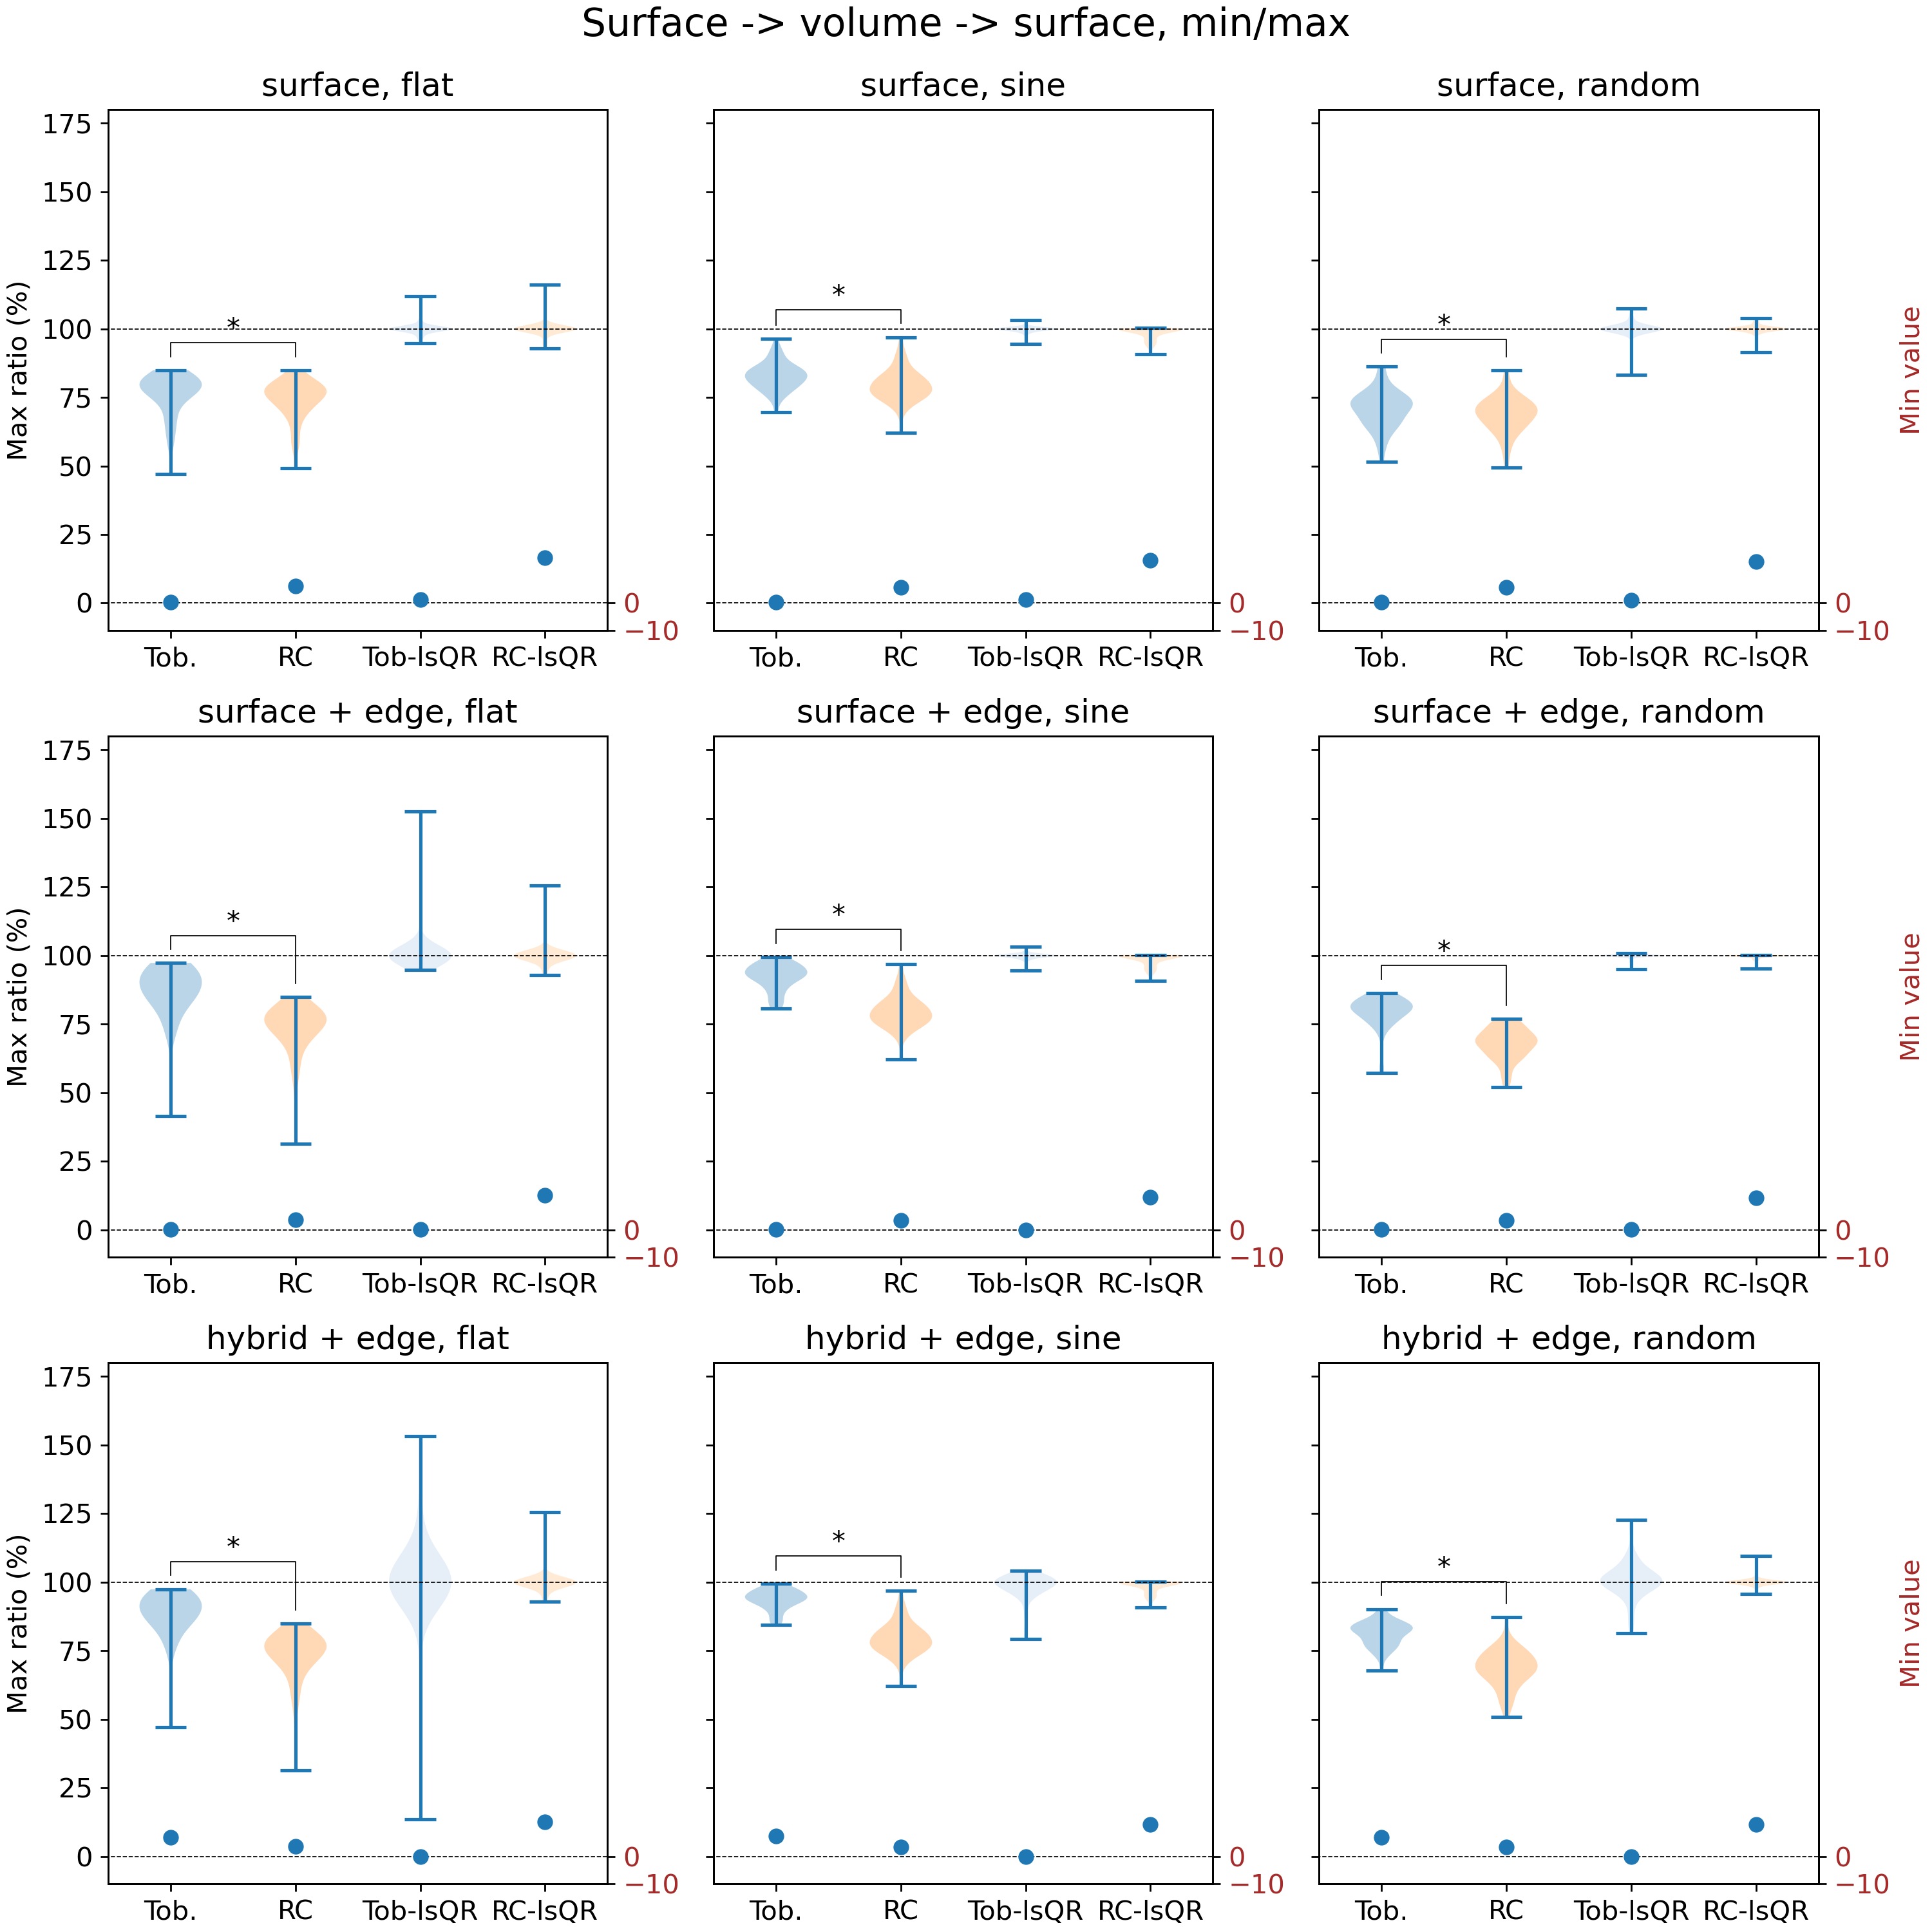
\includegraphics[width=\textwidth]{SVS_minmax}
\caption{Maximum and minimum values, surface-volume-surface projection. Greater variability in these metrics were observed for all methods than in the corresponding volume-surface-volume analysis. Peak signal intensity was marginally higher with Toblerone's surface projection than RC; the difference in performance increased for Toblerone's edge scaling or hybrid projection cases. The lsQR methods did not produce negative values, though their maximum values did exceed reference. * denotes a paired $t$-test result with $p\leq $ 0.001.}
\label{SVS_minmax} 
\end{figure}

Figure \ref{SVS_minmax} shows maximum and minimum signal values for the surface-volume-surface projection test. Referring to the left hand scale on each plot, peak signal values were marginally higher with Toblerone's surface projection than with RC. The use of edge scaling or the hybrid projection, further increased peak signal values for that method. The lsQR methods exhibited some instability, sometimes producing peak signal values greater than 100\% of reference. All comparisons  between Toblerone and RC met the significance threshold. 

\section{Discussion}
Toblerone's surface projection (between volume and surface space only) produced broadly similar results to the RC method in all experiments, with a small and statistically significant improvement in performance (lower RMS error, higher peak signal values). These findings provide reassurance that the principles on which Toblerone's projection have been built are appropriate and confirm that the surface projection could be used as a like-for-like replacement for the RC method. 

Notwithstanding the fact that a comparison between Toblerone's hybrid projection and the RC method is not on like-for-like terms, the results of said comparison showed large and significant advantages for the former. The difference in performance was especially notable  when projecting data that had been simulated with both cortical and subcortical components, as would be the case with ASL data for example (an intended use case). The greatest differences in performance were observed when comparing the RC method to Toblerone's hybrid projection in volume-surface-volume sense: a reduction in RMS errors in the range of 15\% was obtained. Furthermore, Toblerone's distribution across subjects of all metrics (RMS error, maximum value) was often tighter than the equivalent RC distribution, suggesting that the method is consistent and robust. 

All variants of Toblerone and the RC method exhibited high numerical stability compared to the lsQR method, as evidenced by the minimum and maximum values of round-trip projected data which were often outside of the range of ground truth for the latter. Although lsQR often performed extremely well in an aggregate sense (RMS error), particularly when solving the over-determined case of surface to volume projection, the penalty for this was regions of high local instability in which erroneous values were returned. These findings are noteworthy in light of the findings of Lonjaret \textit{et al.} \cite{Lonjaret2017}, who noted that an inverse approach for volume to surface projection is challenging due to the highly under-determined nature of the system. For neuroimaging applications, the potential for such numerical instability within an analysis pipeline would likely be unacceptable. 

\section{Conclusion}

A new framework (Toblerone) for the projection of volumetric data onto the cortical surface has been presented. The core of this makes use of a geometric approach that is similar to that adopted by the ribbon-constrained method used by the HCP, and an evaluation of the two methods on this basis using simulated data found that they performed similarly (with a small and statistically significant advantage in Toblerone's favour). As such, Toblerone could feasibly be used to perform surface-volume projection of arbitrary data. 

Nevertheless, the more important contribution made in this chapter is in providing a foundation for the combined surface and volumetric inference framework that will be introduced in chapter \ref{svb_chapter}. In preparation for this, the concept of hybrid space has been introduced: a space of inference that treats the cortex and subcortex differently and enforces signal separation between the two. In light of this, the novel value of Toblerone's projection framework is that it permits projection of data between the volume and hybrid spaces. 




